\documentclass[master.tex]{subfiles}
 
\newcommand{\meanxy}[1]{\left<#1\right>_{z,y}}
\newcommand{\Tflow}[0]{\overline{\Gamma}}

\begin{document}



\chapter{Effect of Polarization Equation Linearizations on tokamak edge turbulence}\label{sec:polarization_equation_evaluation}

\section{Introduction}
In both gyrokinetic and gyrofluid models the polarization equation plays a central role and the nonlinear nature is often approximated because of the large computational effort associated with the numerical schemes and the assumption that the amplitudes of turbulent fluctuations are much smaller than the background. This may hold for the core plasma but certainly not for the edge region where high background gradients are observed which lead to relatively high amplitude fluctuations if dense \textit{material} is transported from the core region of the separatrix into the \ac{SOL}. For instance the GYSELA polarization equation assumes a equilibrium density $n_0(r)$ where $r$ is to be identified with the $x$-direction \cite{GYSELACODE}. This comes close to linearization 3. The XGC1 code uses a similar approach \cite{XGC1Code}. The following results should give some insight on the effects of the different linearizations. It should be noted that this is not an extensive parameter study and considering the amount of parameters (>10) there could exist various other effects that are not represented by the particular parameters used in the following evaluation.

% The GENE code evaluates the non-linearity but the authors claim that it only has an effect if the electron Debye length $\lambda_{De}$ is comparable to the electron gyro radius $\rho_e$ which in a tokamak is not the case.

\section{Simulation Setup}

The evaluation of the linearizations is done on a 8x128x512 grid with $h_x$ and $h_y=1.0$ (low resolution) and on a 8x256x1024 grid with $h_x = h_y=0.5$ (low resolution). Two parameter sets are tested (for both resolutions). Both sets share the same parameters expect for the perpendicular hyperviscosity $\nu_\perp$:
\begin{itemize}
    \item $\Delta t$: 0.01
    \item $\hat{c}$: 5.0
    \item $\hat{\epsilon}$: 27000.0
    \item $\mathcal{K}_0$: 0.02
    \item $magnetic Shear$: 1.2
    \item $\delta$: 0.015
    \item $\nu_{\parallel}$: 0.2
    \item core Density: 1.2
    \item edge Density: 0.13
\end{itemize}
For the first parameter set $\nu_{\perp} = 0.64|0.04$ (low|high) and for the second set $\nu_{\perp} = 0.96|0.06$. The change of $\nu_\perp$ for the low and high resolution was chosen this way because the term is used to cut off high frequency modes in perpendicular direction. But at a finer resolution in that direction it is not necessary anymore to cut off these modes. Since we are using the fourth derivative in each direction for each direction we get a factor of 4 (in the Fourier-space) and because of that reduce $\nu_\perp$ by $\frac{1}{16} = \frac{1}{4\cdot4}$ to $\nu_\perp = 0.04|0.06$. $\nu_\parallel$ stays untouched since we didn't change the resolution in z-direction \footnote{It should be noted though that through magnetic shearing there could actually be an effect from higher perpendicular resolution on the parallel direction} \newline
The simulation is run on \ac{TV} node using the GPU implementations of the \ac{SOR}-solver and gyroaveraging operator. Both versions are run for 150,000 iterations and full data output is created every 15,000 iterations. Combined qunatities (Turbulent Flow, Parallel Kinetic Energy...) are recorded every 20 iterations.


\section{Equilibrium State}
At first the simulation develops strong turbulence and high fluctuations which result in an outburst of "material" (i. e. the total density decreases). Afterwards the simulation approaches a steady state where the state variables only vary little and a typical energy cascade forms. This equilibrium behavior can be seen by looking for instance at temporal evolution of the parallel kinetic energy (\autoref{sec:polar_parallel_velocities}) or the total density both restricted to the core and \ac{SOL} plasma (in/out separatrix) . The data suggests that a stable regime is reached after about 100,000 iterations\footnote{This is not the case for each and every presented simulation but it is at least fairly stable after 100,000 iterations. Future studies should increase the iterations run to at least 250,000.}. The idea now is to compare mean values over the simulation time where a equilibrium state has been reached. 

\begin{figure}[!hbtp]
    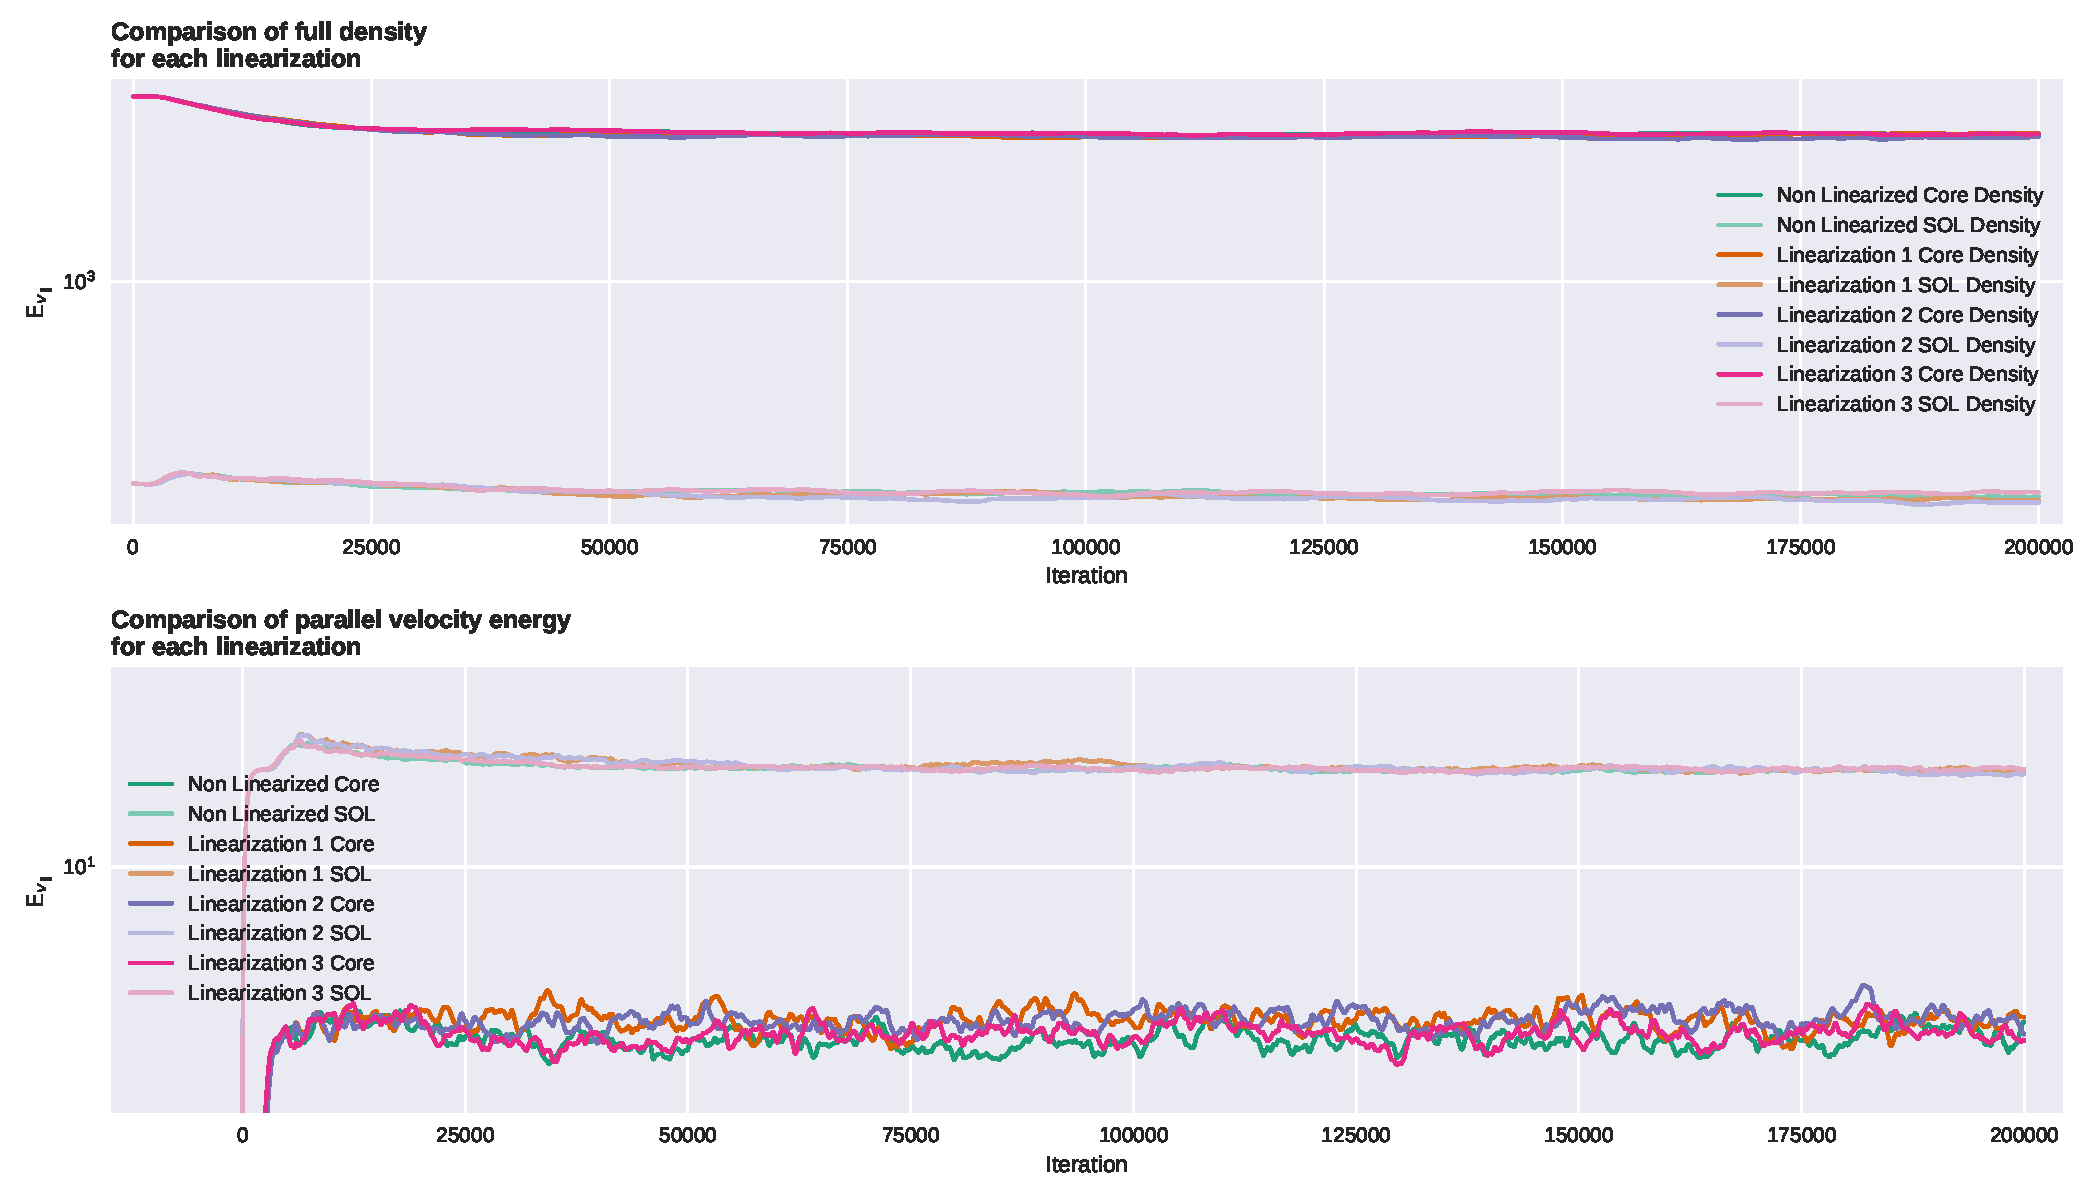
\includegraphics[width=\linewidth]{pdfs/equilibrium_state_low.pdf}
    \caption{Temporal evolution of ($E_n$ \autoref{sec:fluid-dynamics}) and the parallel kinetic energy (see \autoref{sec:polar_parallel_velocities}) both restricted to Core and \ac{SOL} region. After 80,000 iterations a steady state is reached.}
\end{figure}


\begin{blockquote}
    The errors attached to the mean values are calculated via the standard derivation but do not represent the error of multiple simulations or the response to disturbed input parameters but rather give an idea about the size of fluctuations in the equilibrium state.
\end{blockquote}
    
\section{Evaluation}
To compare the different linearizations defined in \autoref{sec:polarization-linearizations} the mean turbulent flow in the steady state regime is compared for the core and \ac{SOL} plasma. Further on the zonal potential  $\meanxy{\phi_e}$, the zonal flow ($\partial_x \meanxy{\phi_e}$), the vorticity ($\partial_{xx}\meanxy{\phi_e}$) and the zonal turbulent flux ($\left<\Gamma^*\right>_{z,y}$) are compared and finally the parallel kinetc velocity is taken into account.


\section{Turbulent Flow}
The turbulent flow is calculated as it is defined in \autoref{sec:simulation_quantities}. The turbulent flows (Core/\ac{SOL}) for the whole simulation are displayed in \autoref{fig:turbulent-flow-low} on a semi logarithmic grid. From this figure one can already see that there is no apparent difference for the turbulent flows in regard to the linearizations for this particular parameterset.
\begin{figure}[!htbp]
    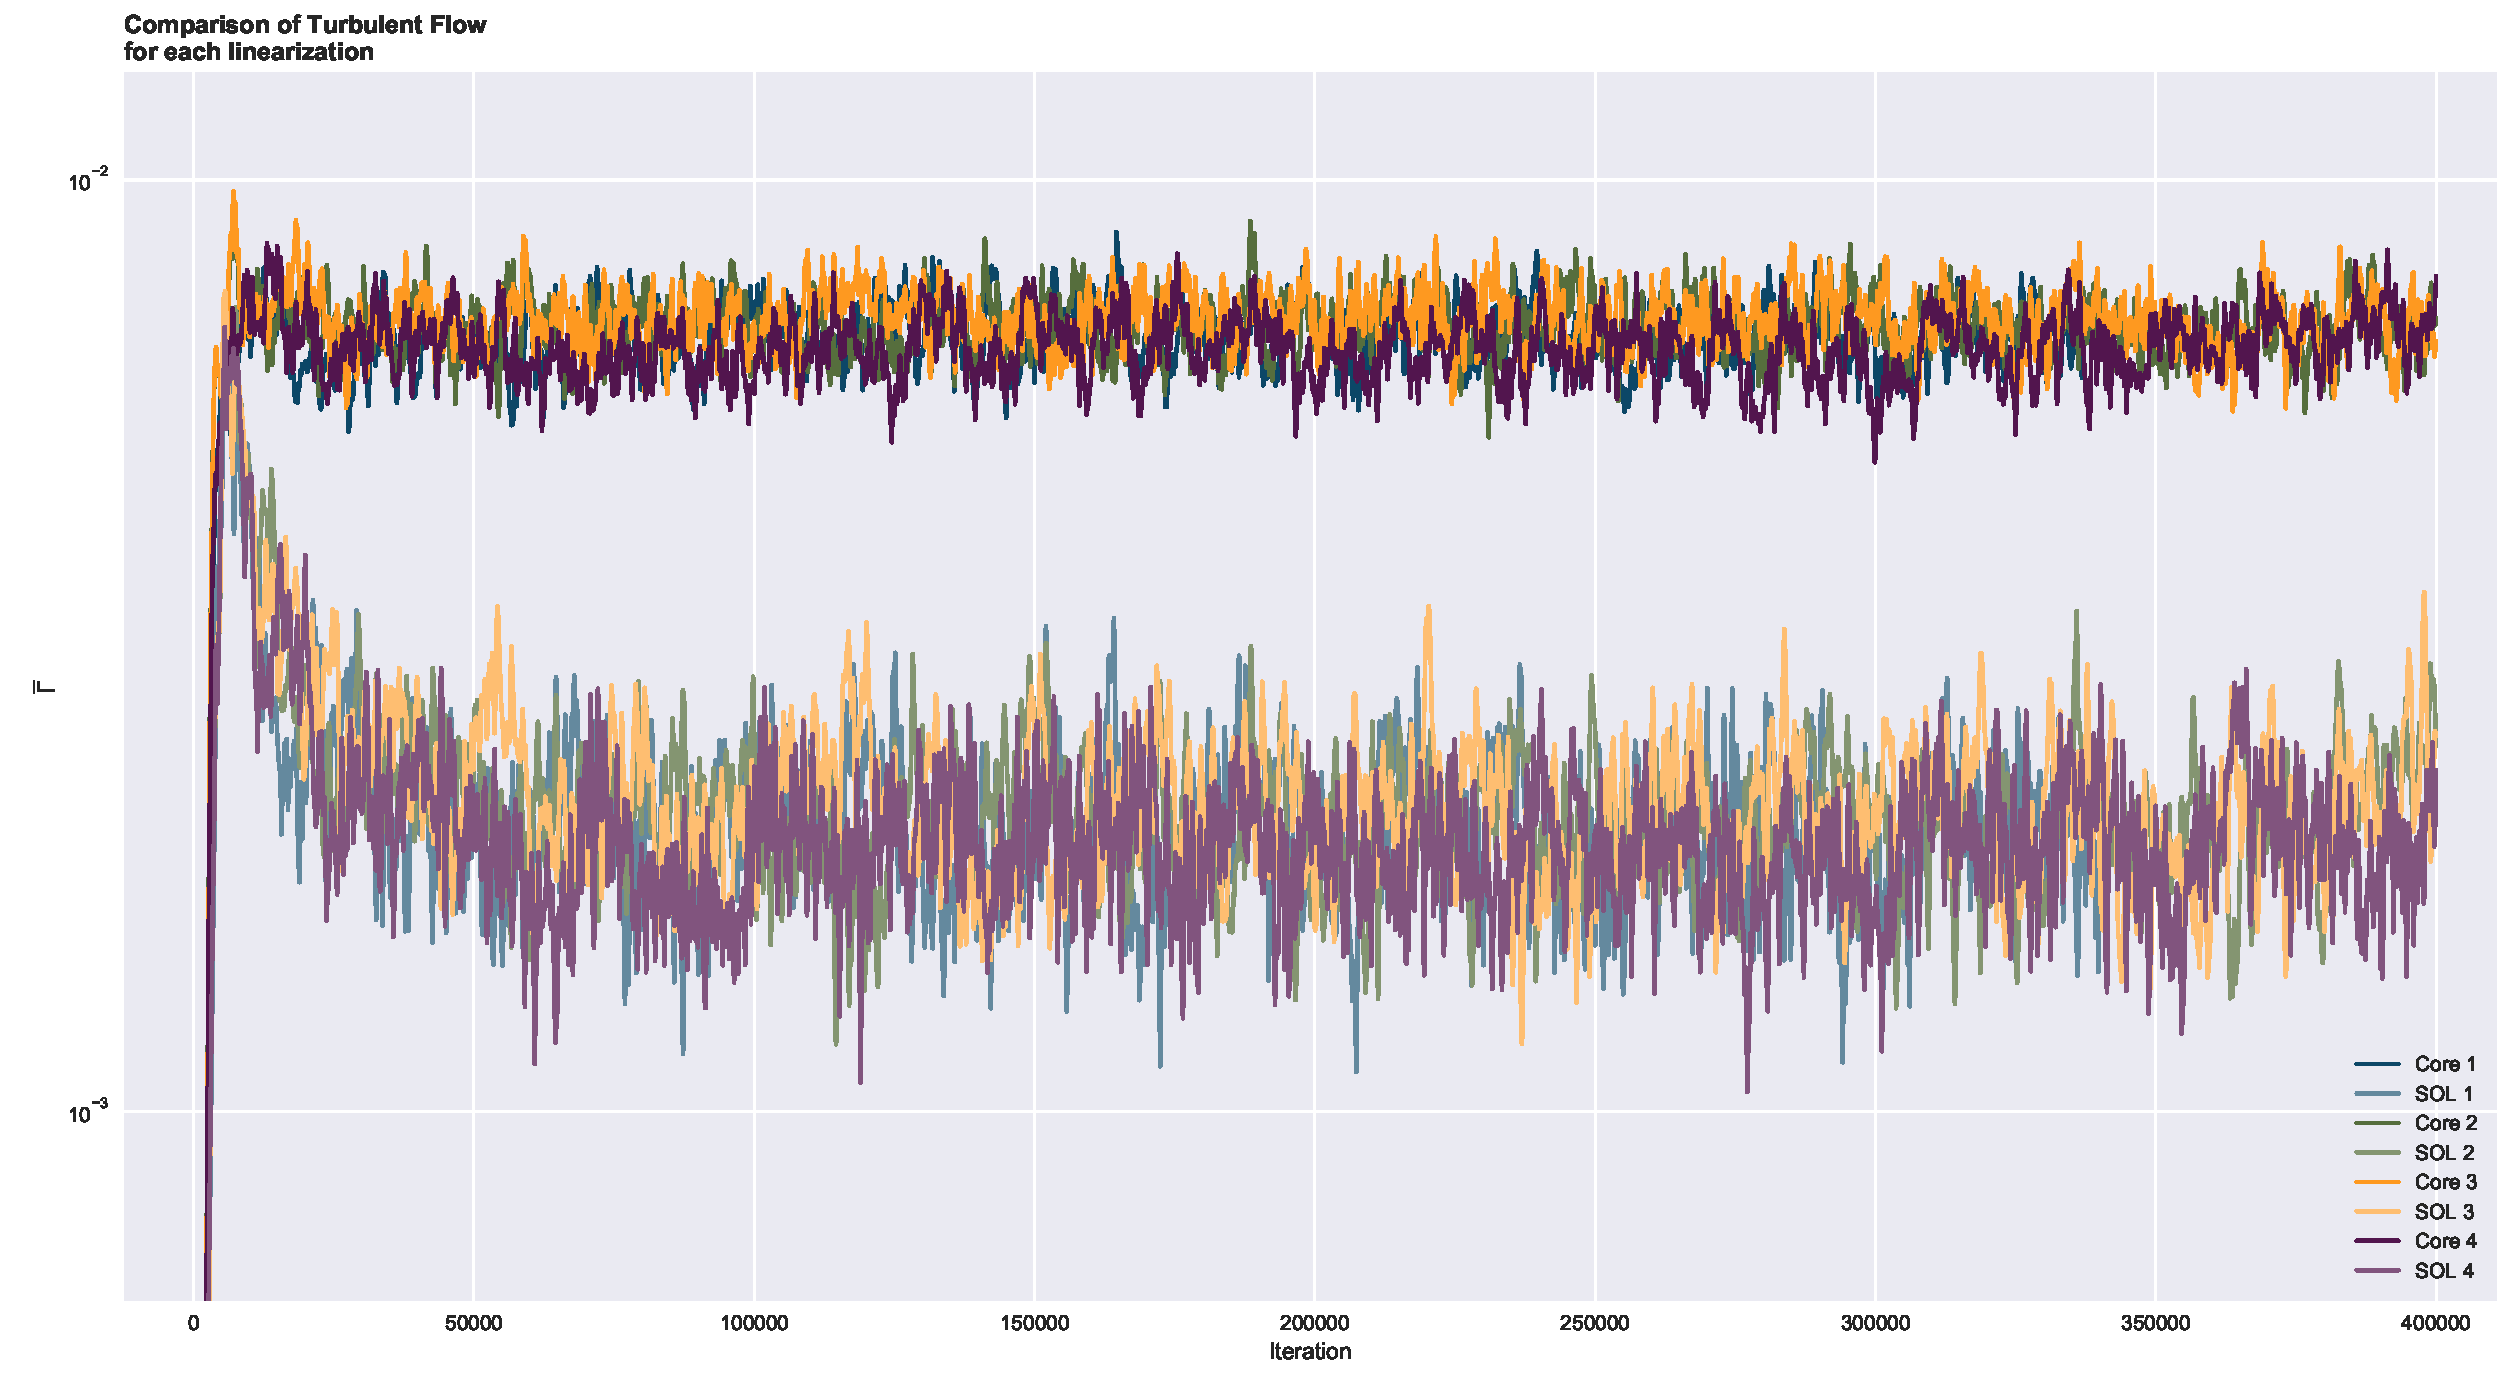
\includegraphics[width=\linewidth]{pdfs/turbulent-flow-low.pdf}
    \caption{Turbulent flow split into Core and \ac{SOL} region for each linearization. The lighter colors represent the \ac{SOL} parts.}
    \label{fig:turbulent-flow-low}
\end{figure}
\autoref{fig:turbulent-flow-low-means} shows the mean value of $\Tflow_{Core}$ and $\Tflow_{SOL}$ from 70,000 to 150,000 iterations. There may be a small indication that $\Tflow_{Core}$ is a little higher for the constant background (local model) linearizations but considering the magnitude of fluctuations (visualized by the error bars) this seems very far fetched. 



\begin{figure}[!htbp]
    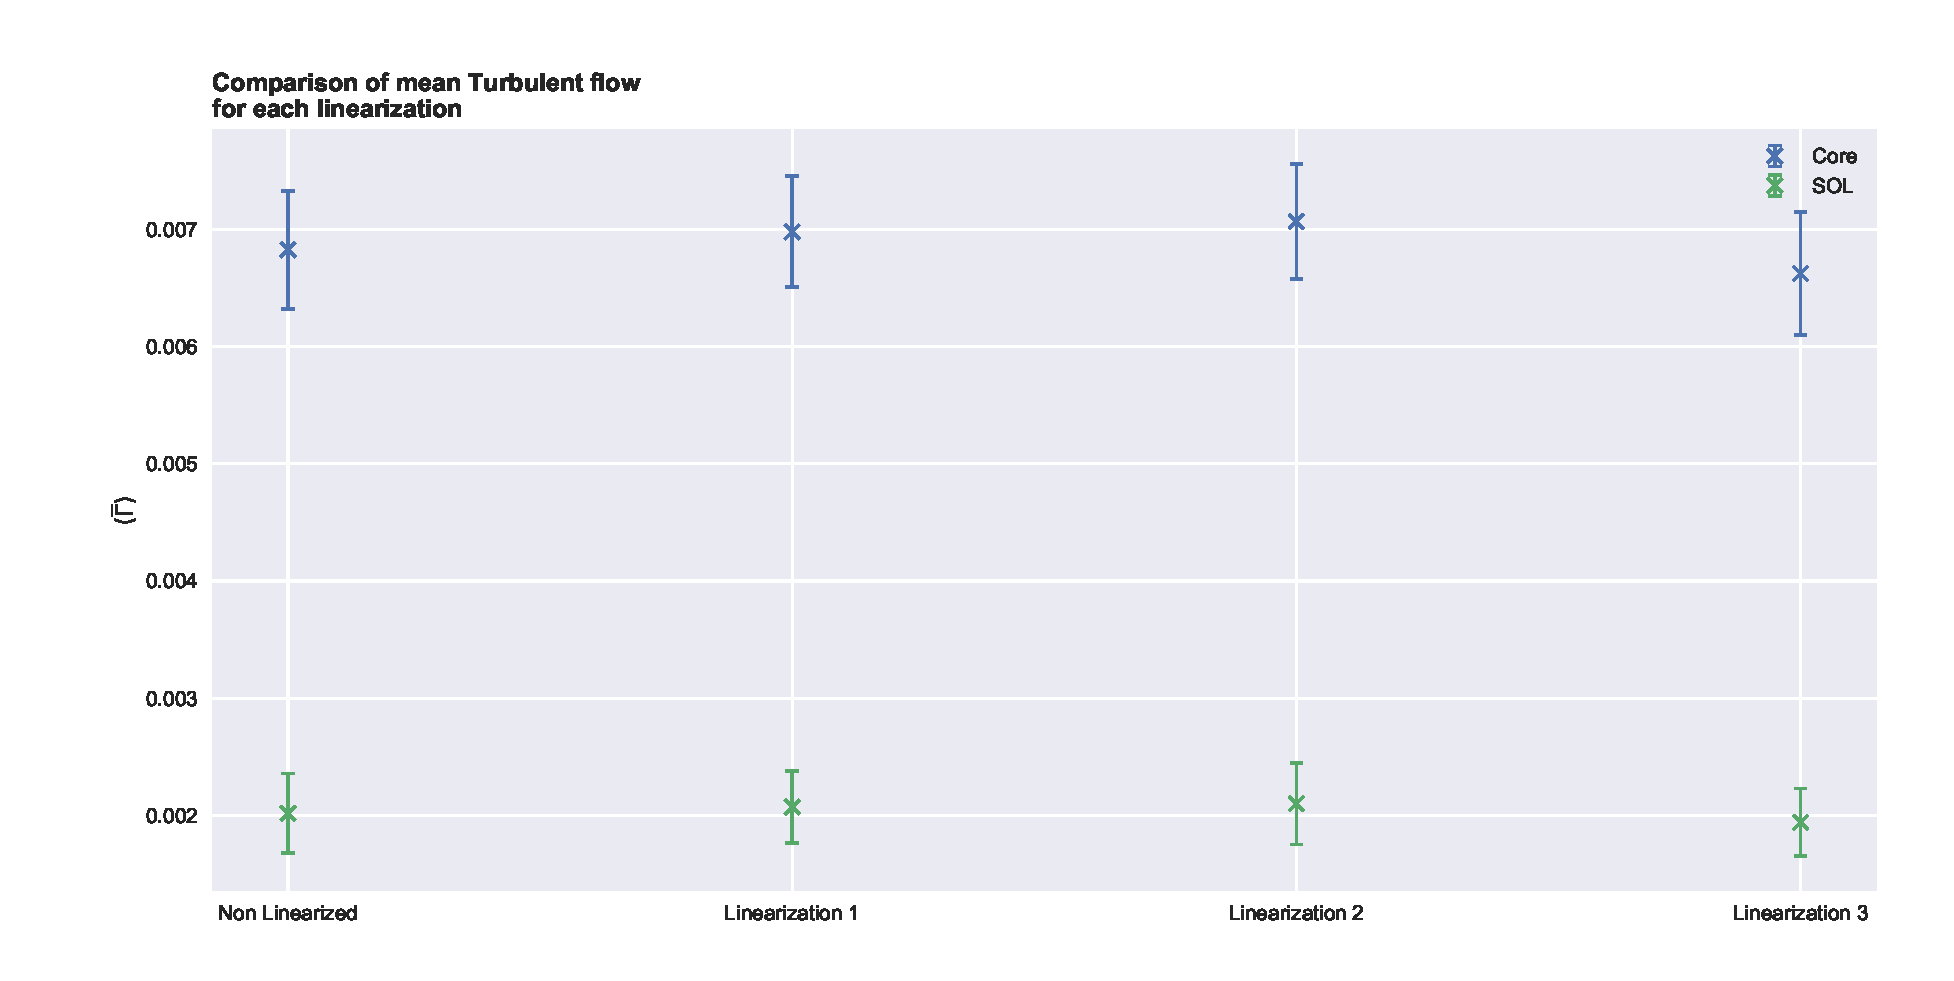
\includegraphics[width=\linewidth]{pdfs/turbulent-flow-low-means.pdf}
    \caption{Mean values of $\Tflow$ after 80,000 iterations. There is no apparent difference visible.}
    \label{fig:turbulent-flow-low-means}
\end{figure}

\section{Zonal Potential}

The same procedure of the previous section is applied to the zonal potential, zonal flow and zonal flow potential (vorticity). The results are shown in \autoref{fig:zonal-potential-low-all}.\\
They form two groups: The non linearized model and the third linearization share distinct features as well as the first and the second. Since the linearization specifically targets the gradient of the densities which is the strongest close to the core plasma, the greatest difference between the linearizations and the non linearized model is observed there. One has to note that on the boundaries numerical artifacts play a major role leading to artificial density gradients explaining for instance the \textit{bump} on the $x_L$ boundary. Looking at the zonal flow the first group generally produces stronger zonal flows in the region of the separatrix ($x\approx 64$). This may have some implications on the formation of a transport barrier in that area.

\begin{figure}[!htbp]
    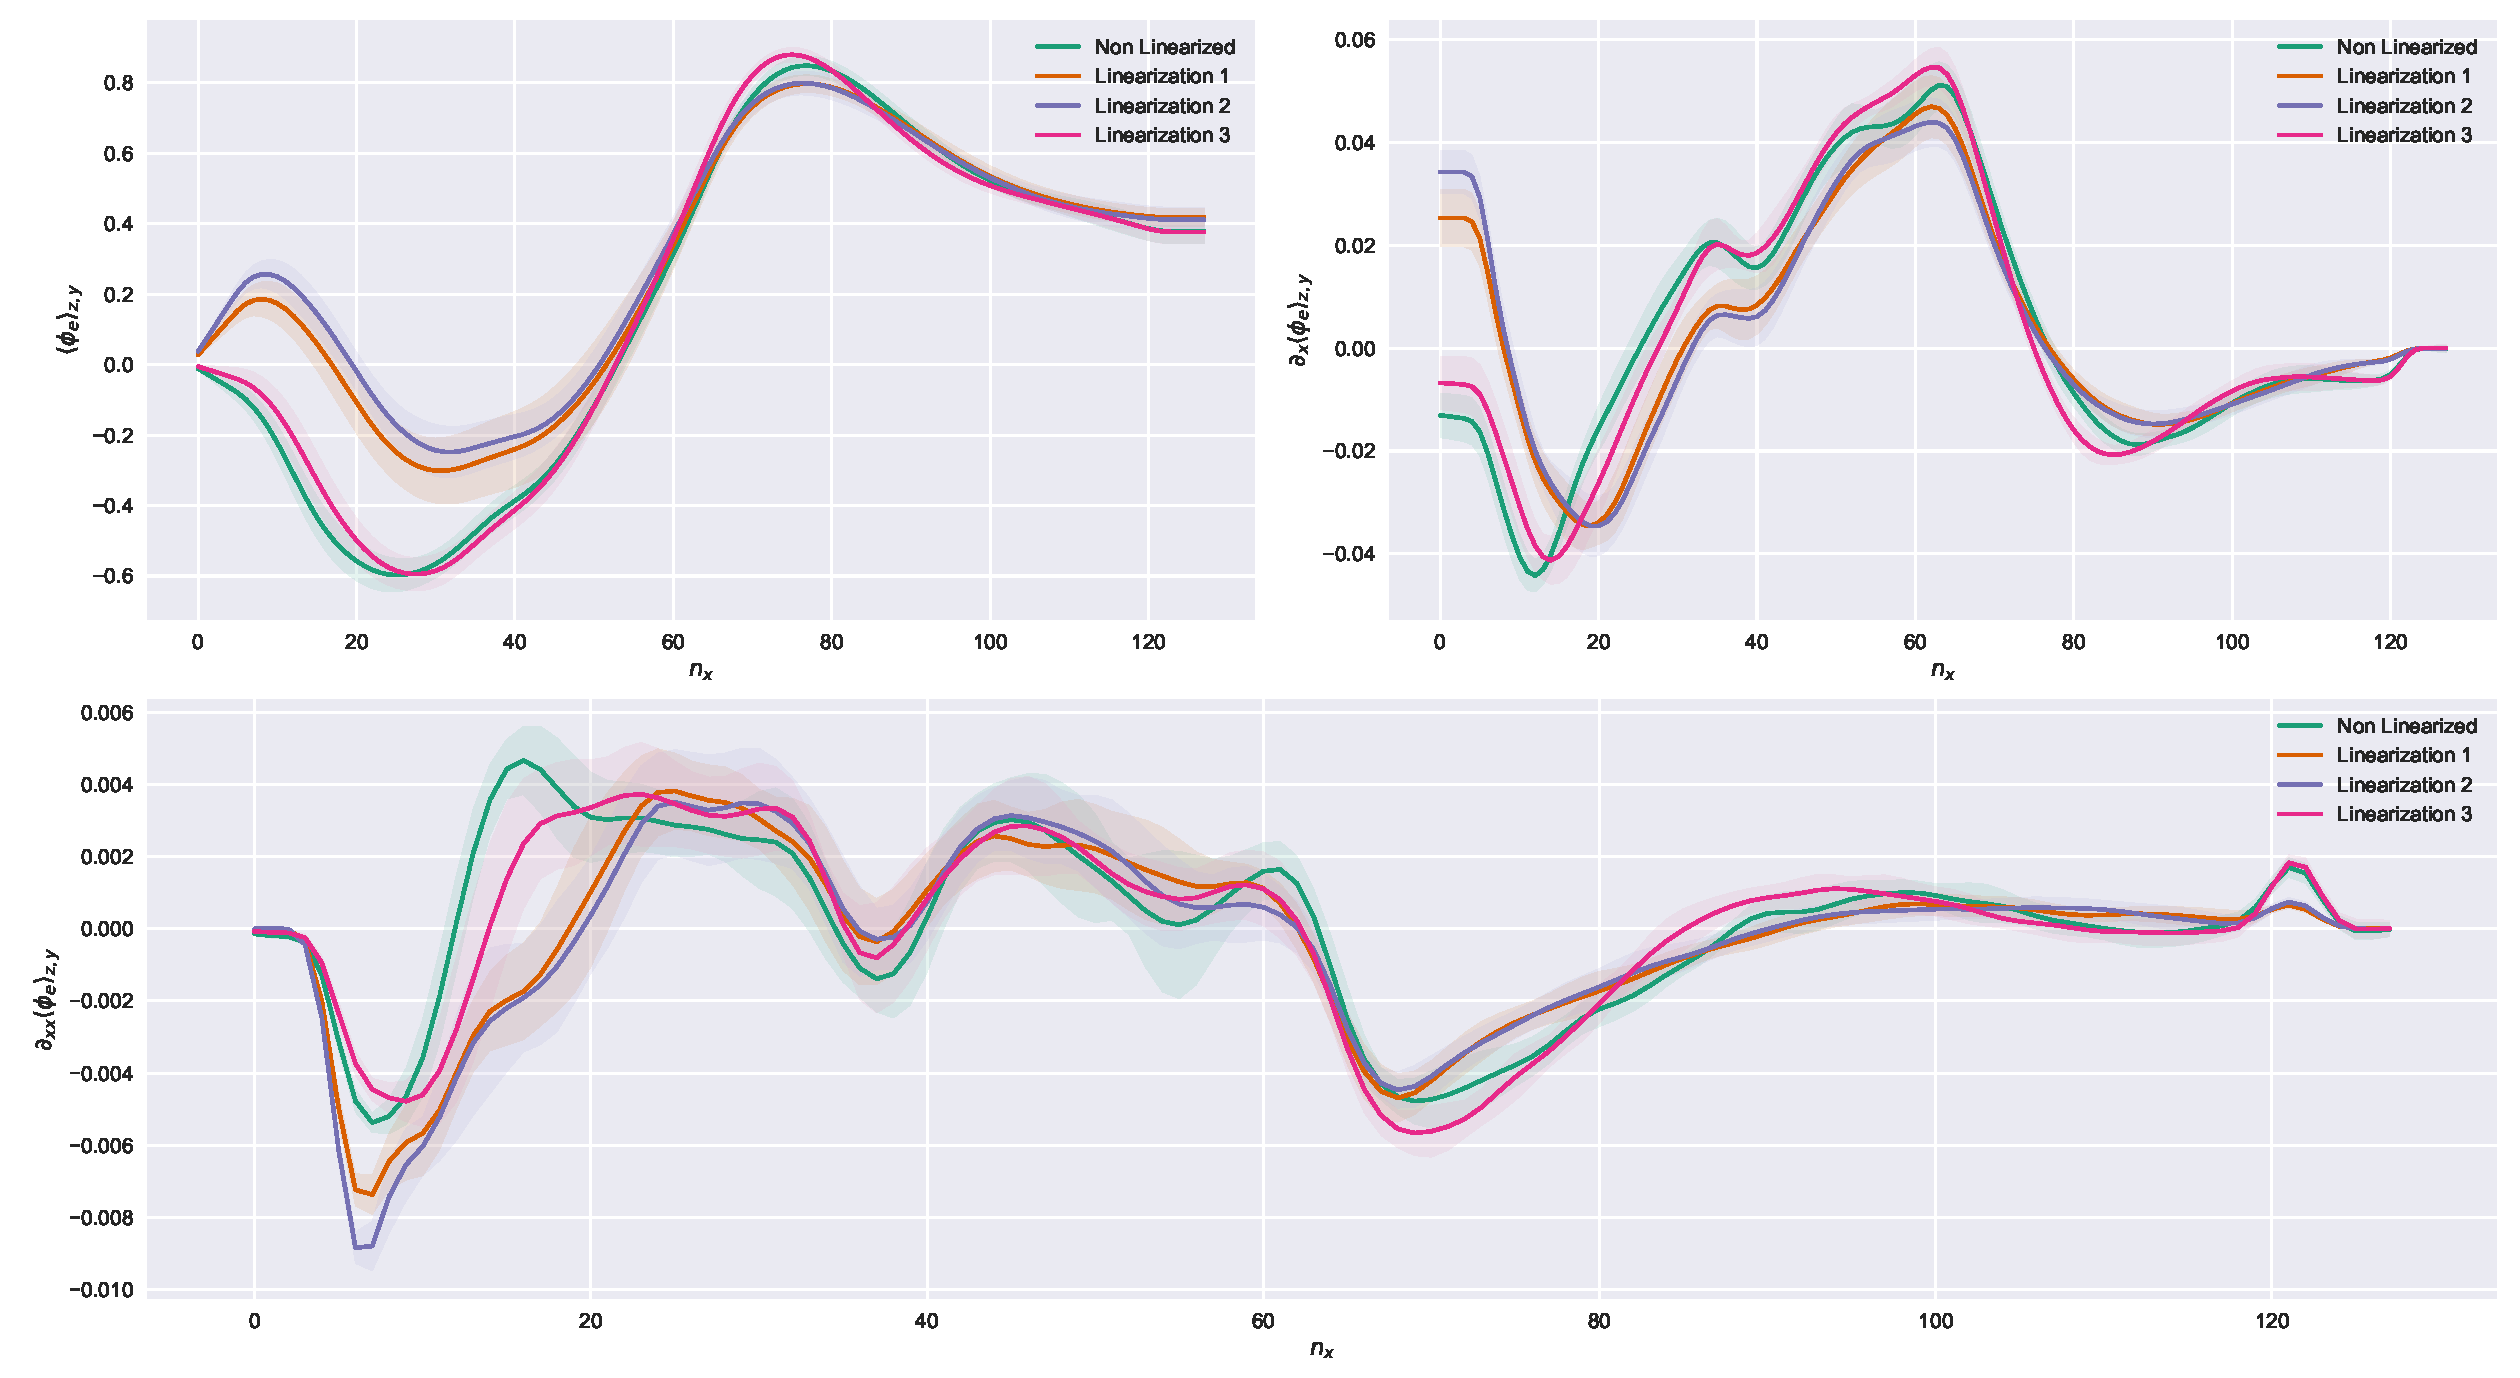
\includegraphics[width=\linewidth]{pdfs/zonal_potential_low.pdf}
    \caption{Mean values of Zonal Potential, Zonal Flow and Zonal Flow Potential of iteration 80,000-150,000. The shaded areas show fluctuations for each case.}
    \label{fig:zonal-potential-low-all}
\end{figure}

\section{Parallel Kinetic Energy $E_{v\parallel}$}\label{sec:polar_parallel_velocities}

To \textit{measure} the influence in the parallel direction it might be helpful to look at the $E_{v\parallel}$ as it is defined in \autoref{sec:fluid-dynamics}.\newline
As in the previous chapters the integration will be restricted to either Core or the \ac{SOL} region. The time evolution of these quantities is shown in \autoref{fig:velocity-energy-low}.

\begin{figure}[!htbp]
    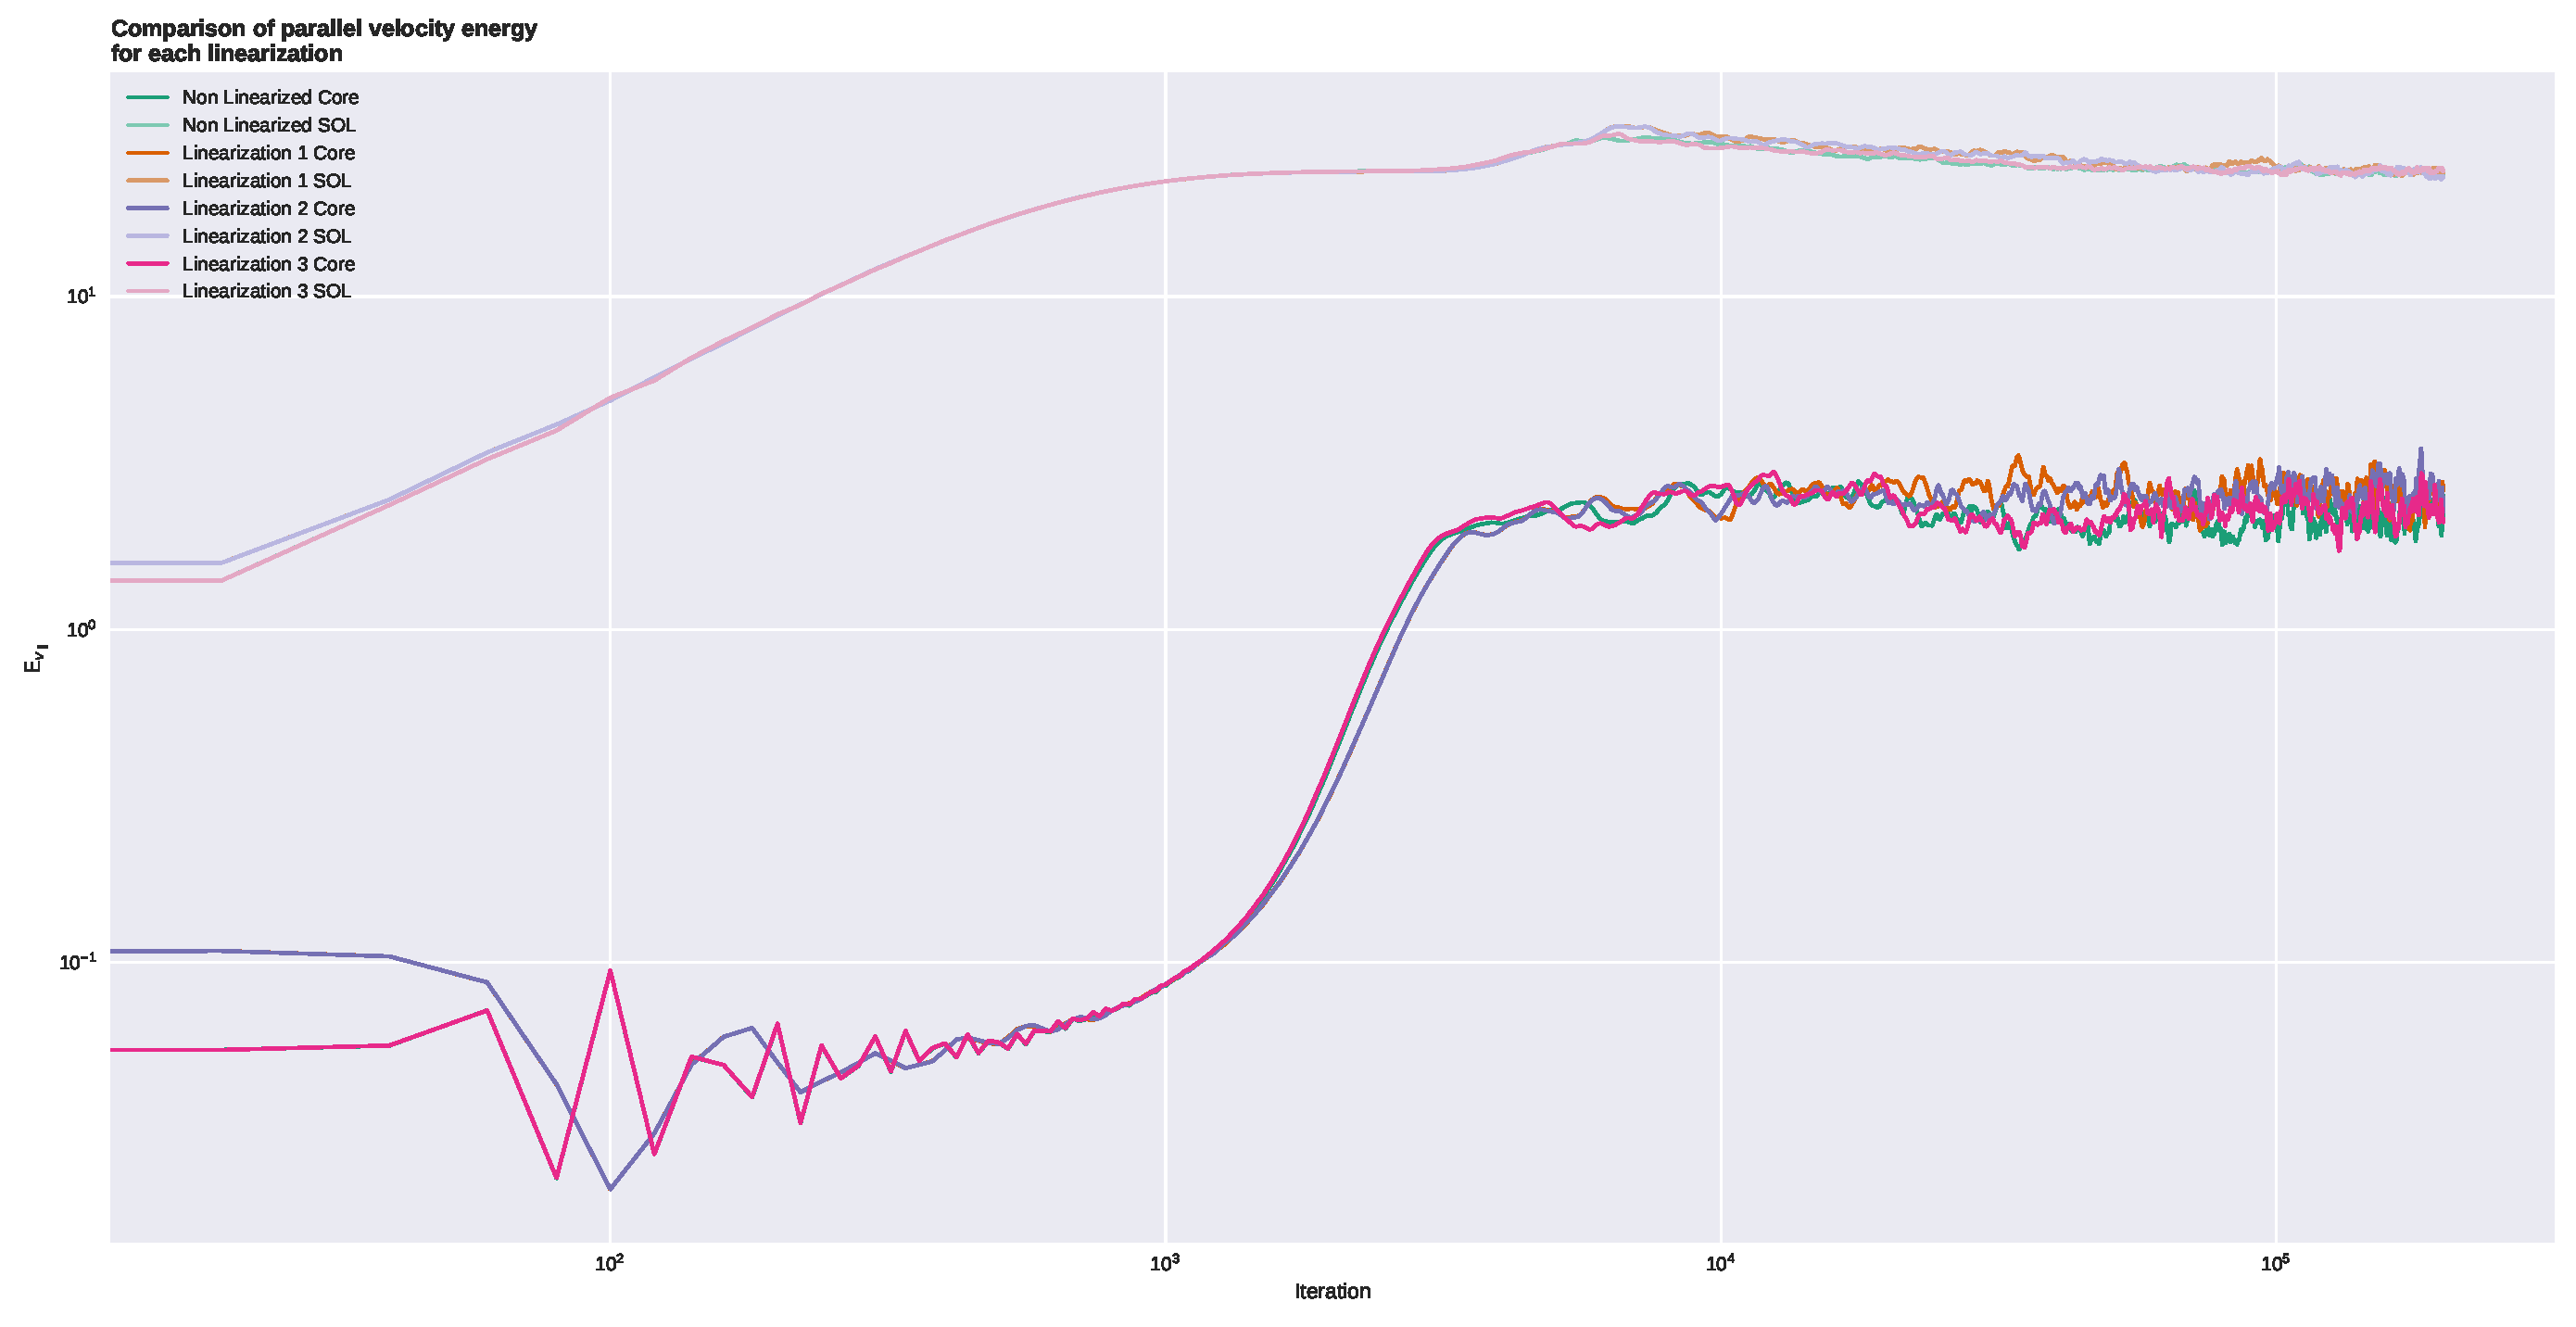
\includegraphics[width=\linewidth]{pdfs/velocity-energy-low.pdf}
    \caption{Time evolution of $\mathrm{E}_{v_\parallel}$ for Core and \ac{SOL} region. This time in a log-log coordinate system.}
    \label{fig:velocity-energy-low}
\end{figure}

The comparison shows no major difference but if one looks at the mean values the splitting into two groups from the previous section is visible again (\autoref{fig:velocity-energy-low-mean}).


\begin{figure}[!htbp]
    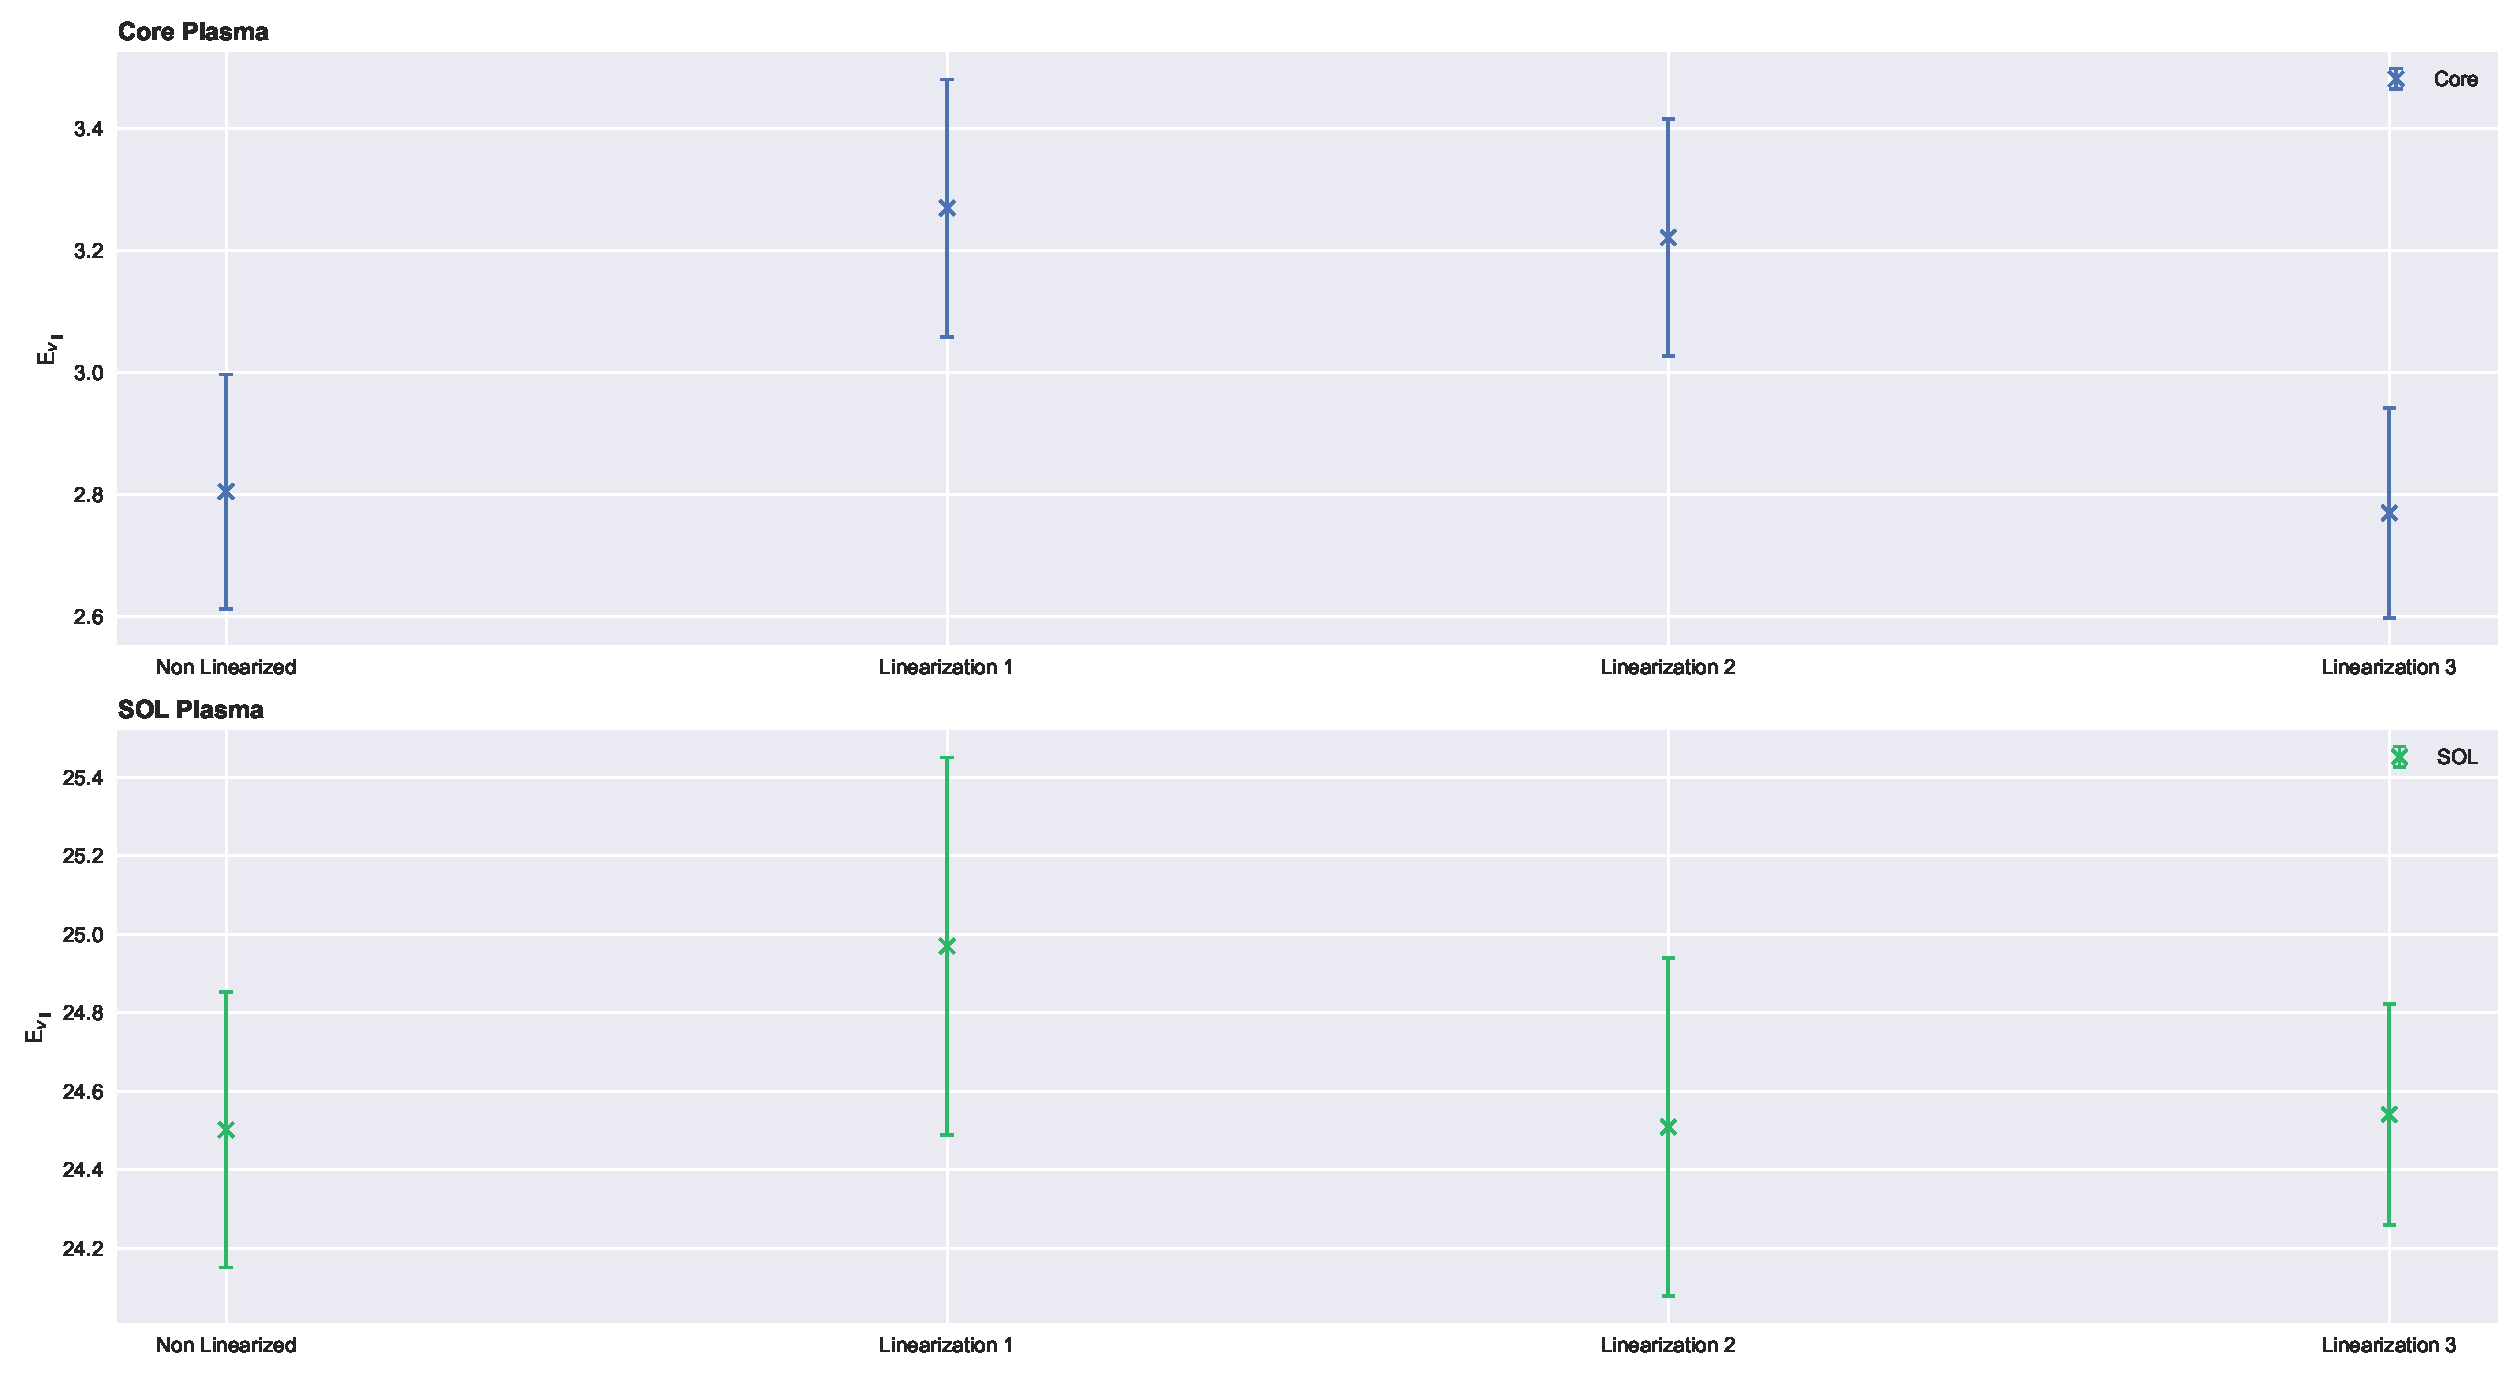
\includegraphics[width=\linewidth]{pdfs/velocity-energy-low-means.pdf}
    \caption{Mean of Velocity Energy from 80,000 to 150,000 iterations}
    \label{fig:velocity-energy-low-mean}
\end{figure}

\section{High resolution Data \textit{(2\textsuperscript{nd} parameter set)}}
The same procedures from the previous sections are applied to a finer grid (8x256x1024; $h_x = h_y = 0.5$). One has to account for a higher resolution by reducing $\Delta t$ to stay in the \ac{CFL} limit. It is also expected that the perpendicular hyperviscosity has to be adjusted to account for the higher resolution in the perpendicular plane because the finer grid now allows higher wave numbers. \newline
\todo{Understand this derivation....}The perpendicular hyperviscosity is realized using the fourth derivative in $x$ and $y$ direction.. \newline
To get a one to one mapping from the lower resolution to the higher resolution turned out to be very difficult because the higher resolution has a great negative impact on the stability. In the following sections two parameter sets are presented where the first tries to achieve a mapping from the lower resolution to the higher and the second one represents a new parameter set with higher viscosities.

\subsection{1\textsuperscript{st} Parameter Set High Resolution}
This parameter set should actually represent resolution scaling but to achieve a stable set it was necessary to reduce $\Delta t$ to $0.001$. Now it would have been necessary to run the simulation for a lot longer time but this was not done here because when looking at the data after 200,000 iterations numerical artifacts are already visible.\newline
For this set only $\Delta t$ and $\nu_\perp = 0.001375$ where changed.\newline
The mean values were taken from iteration 160,000 to 200,000.
\autoref{fig:density-velocity-high-wrong} shows the evolution of full density and velocity. Here one already sees that something unexpected is happening with linearization two. Also some kind of resonance is visible in the parallel kinetic energy. This probably arises from the small timestep for which the timestepper is not stable anymore.

\begin{figure}[!hbtp]
    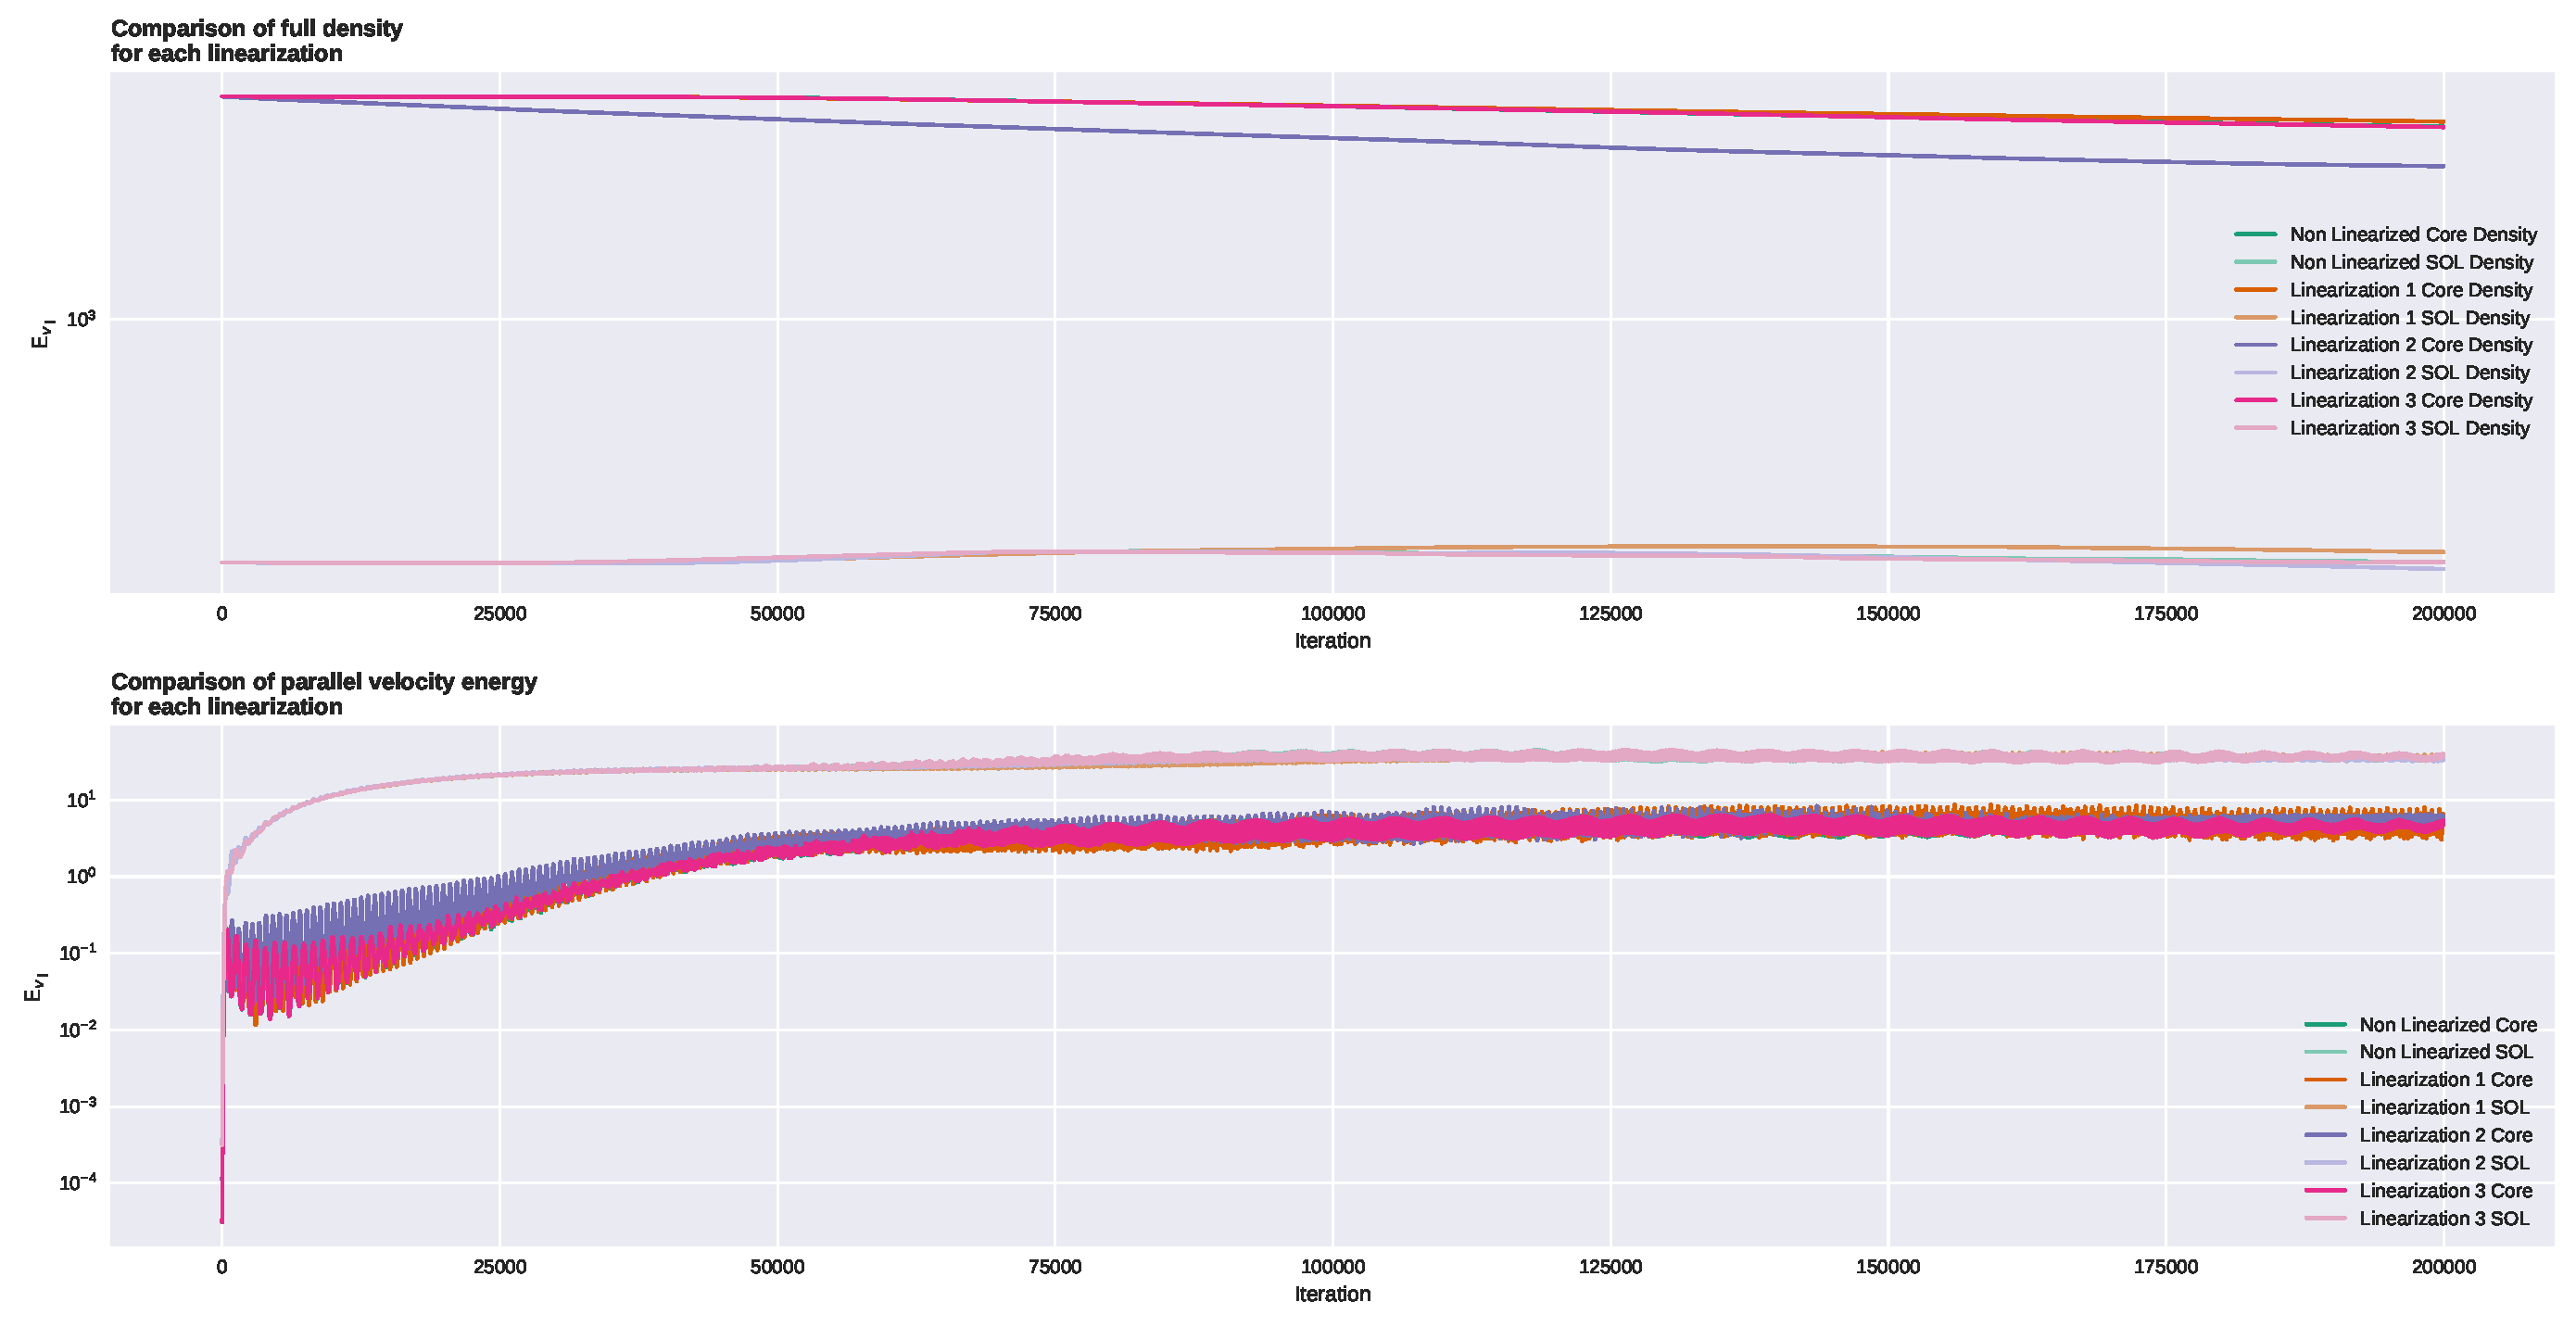
\includegraphics[width=\linewidth]{pdfs/0-11_0-001375/density_vs_velocity.pdf}
    \label{fig:density-velocity-high-wrong}
    \caption{Full density and parallel energy for the 1\textsuperscript{st} parameter set at a higher resolution.}
\end{figure}

\autoref{fig:zonal_profiles-high_wrong} shows the zonal profiles but here the outlier linearization two is clearly visible. Considering the instable nature of this parameter set it is discarded further on and was only presented to show the difficulties involved with resolution scaling for this model and simulation.

\begin{figure}[!hbtp]
    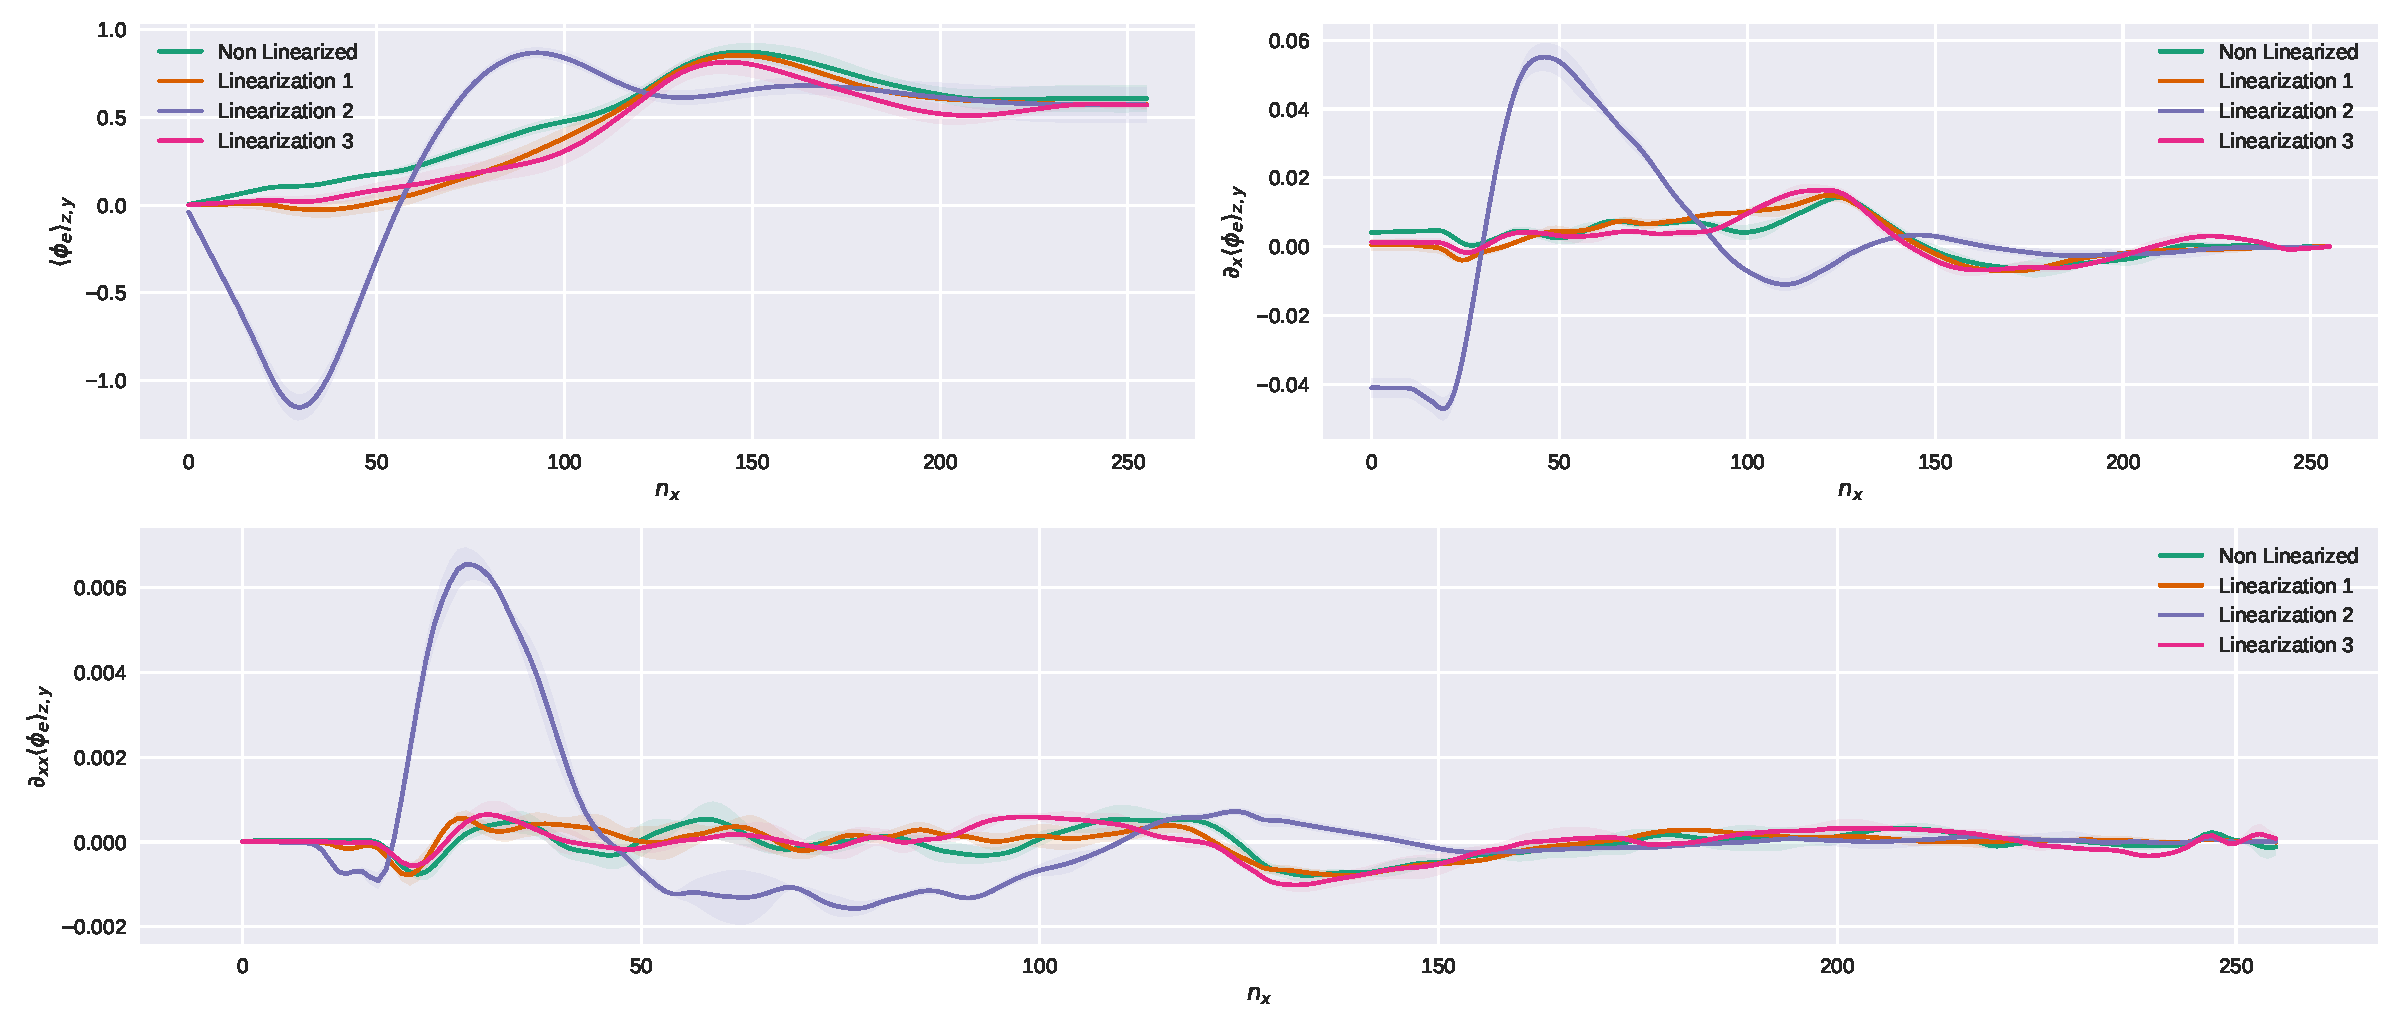
\includegraphics[width=\linewidth]{pdfs/0-11_0-001375/zonal_profiles.pdf}
    \label{fig:zonal_profiles-high_wrong}
    \caption{Zonal profiles for the 1\textsuperscript{st} parameter set at a higher resolution.}
\end{figure}

\subsection{2\textsuperscript{nd} Parameter Set}
A second parameter set was evaluated where $\nu_\parallel = 0.2$ and $\nu_\perp = 0.96$ ($\nu_\perp = 0.06$ for higher resolution). These parameters produce a stable simulation for the higher resolution at $\Delta t = 0.01$. Only the zonal profiles (\autoref{fig:zonal_profiles-high_good}), values for the turbulent flow (\autoref{fig:turbulent-flow-means-high_good}) and the parallel kinetic energy (\autoref{fig:velocity-energy-means-high_good}) are presented here. 





\section{2\textsuperscript{nd} Parameter Set}
The second parameter set only changes for the perpendicular hyperviscosity which is increased to $v_\perp = 0.96 | 0.06$ for $h_x=h_y=1.0|0.5$ respectively.

\subsubsection{Low Resolution (8x128x512 $h_x=h_y=1.0$)}

First the results of the low resolution set are presented in \autoref{fig:low-resoultion-set-2}.

\begin{figure}[!hbtp]
    \textbf{Zonal Profiles, mean Turbulent flows and Parallel Kinetic Energies}\par\medskip
    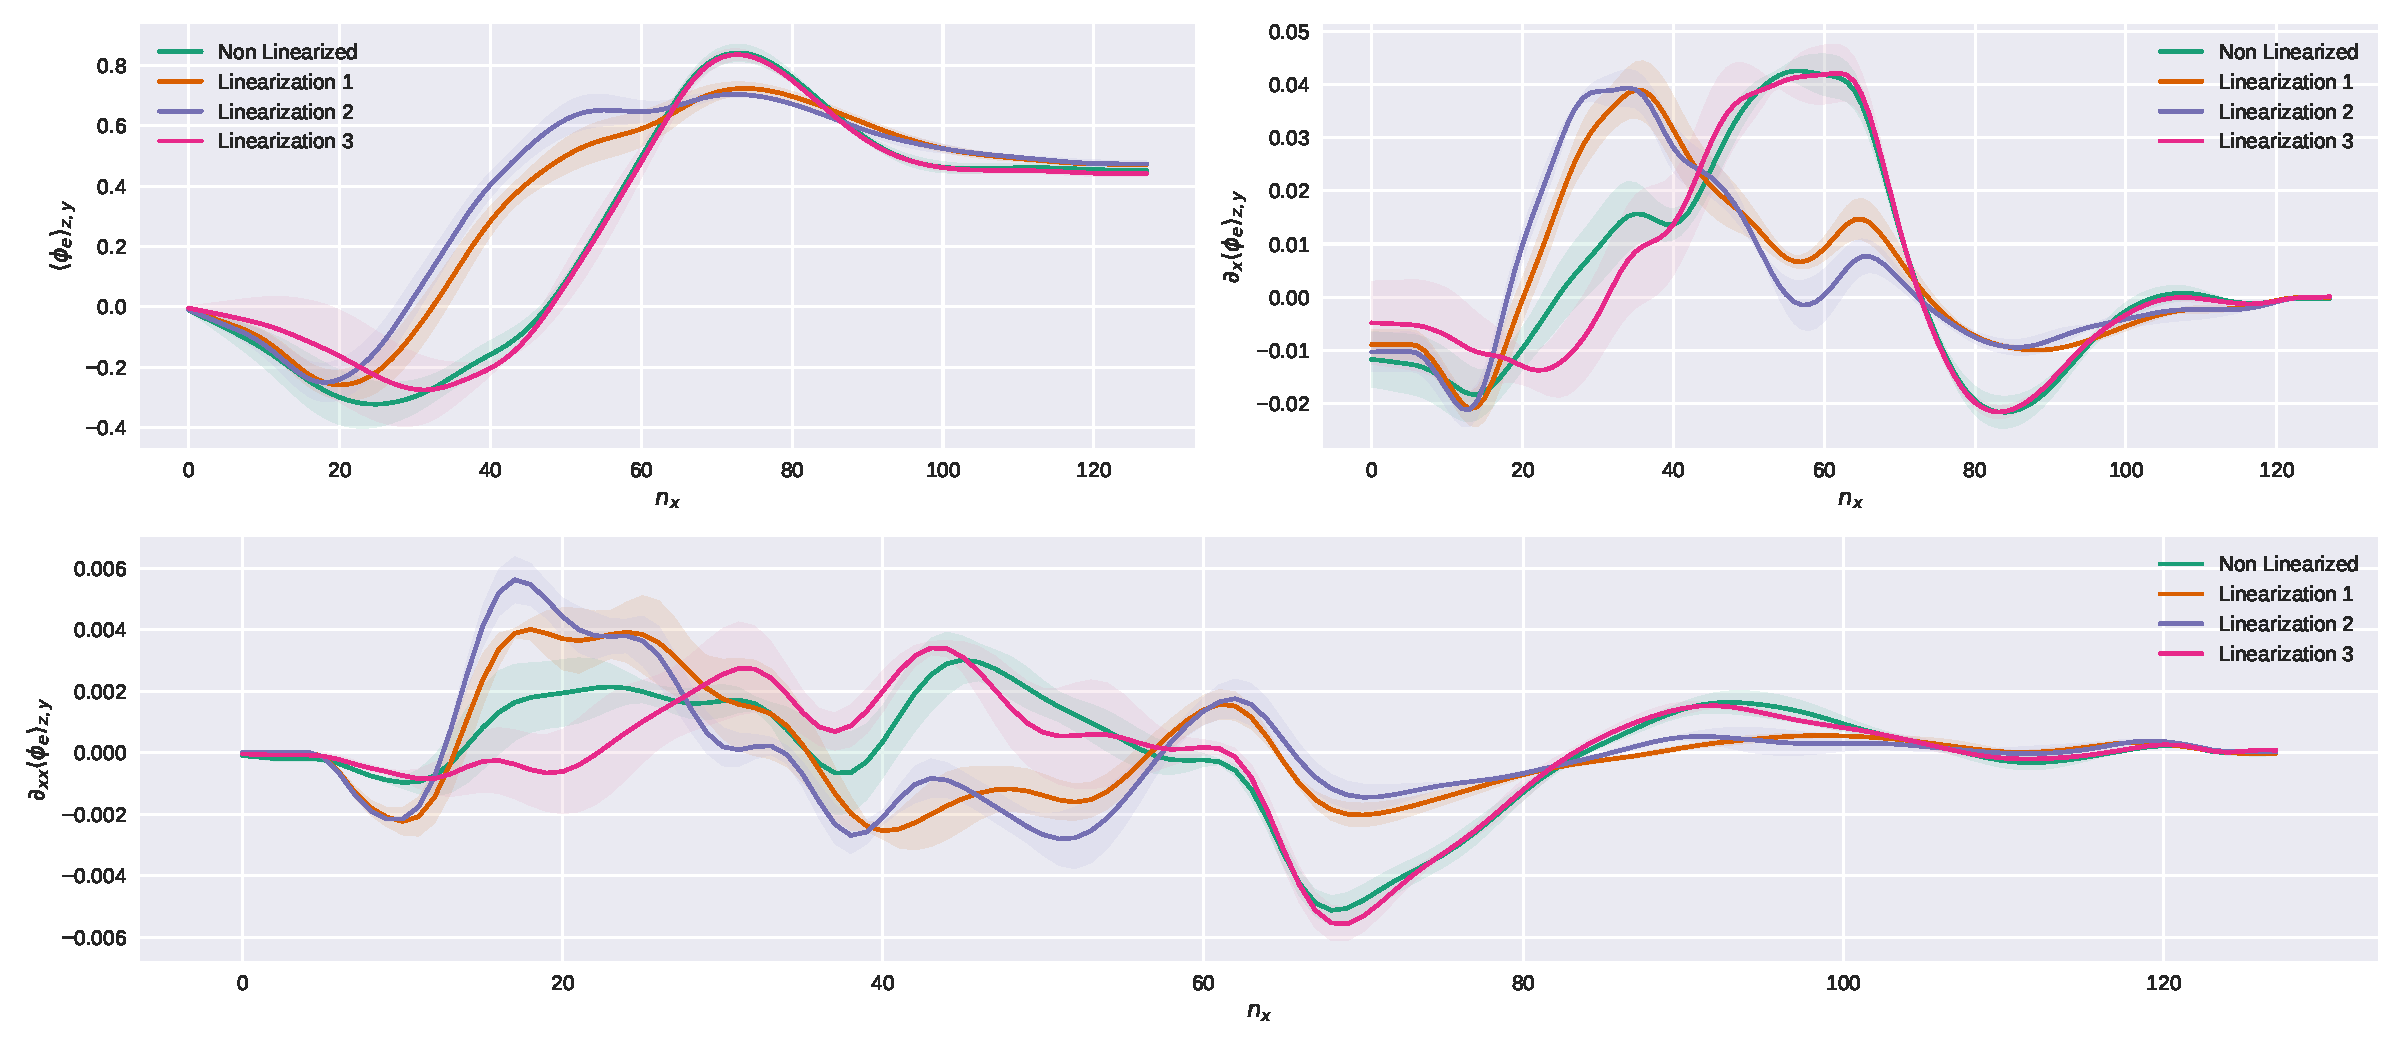
\includegraphics[width=\linewidth]{pdfs/0-2_0-96/zonal_profiles_100000.pdf}
    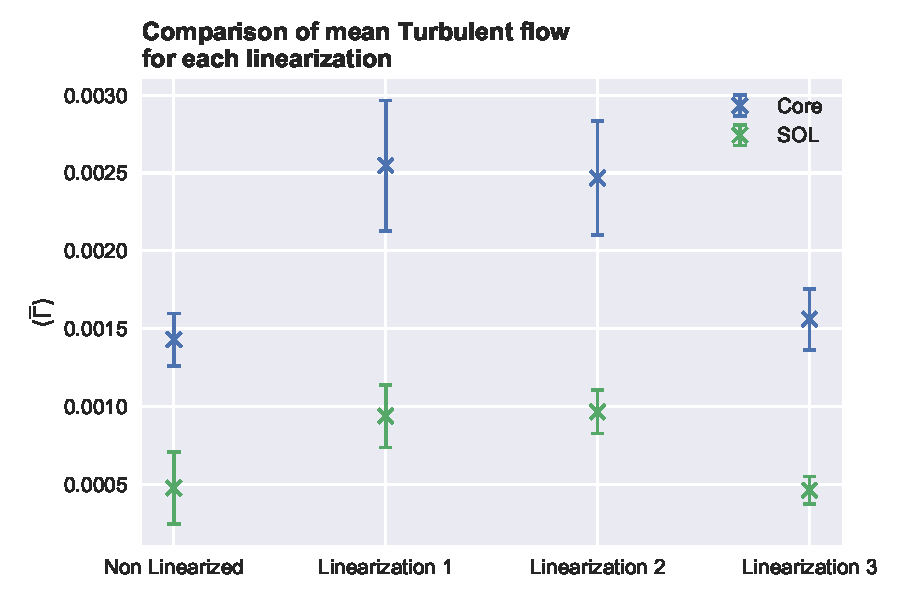
\includegraphics[width=0.5\linewidth]{pdfs/0-2_0-96/turbulent_flow_means_100000.pdf}
    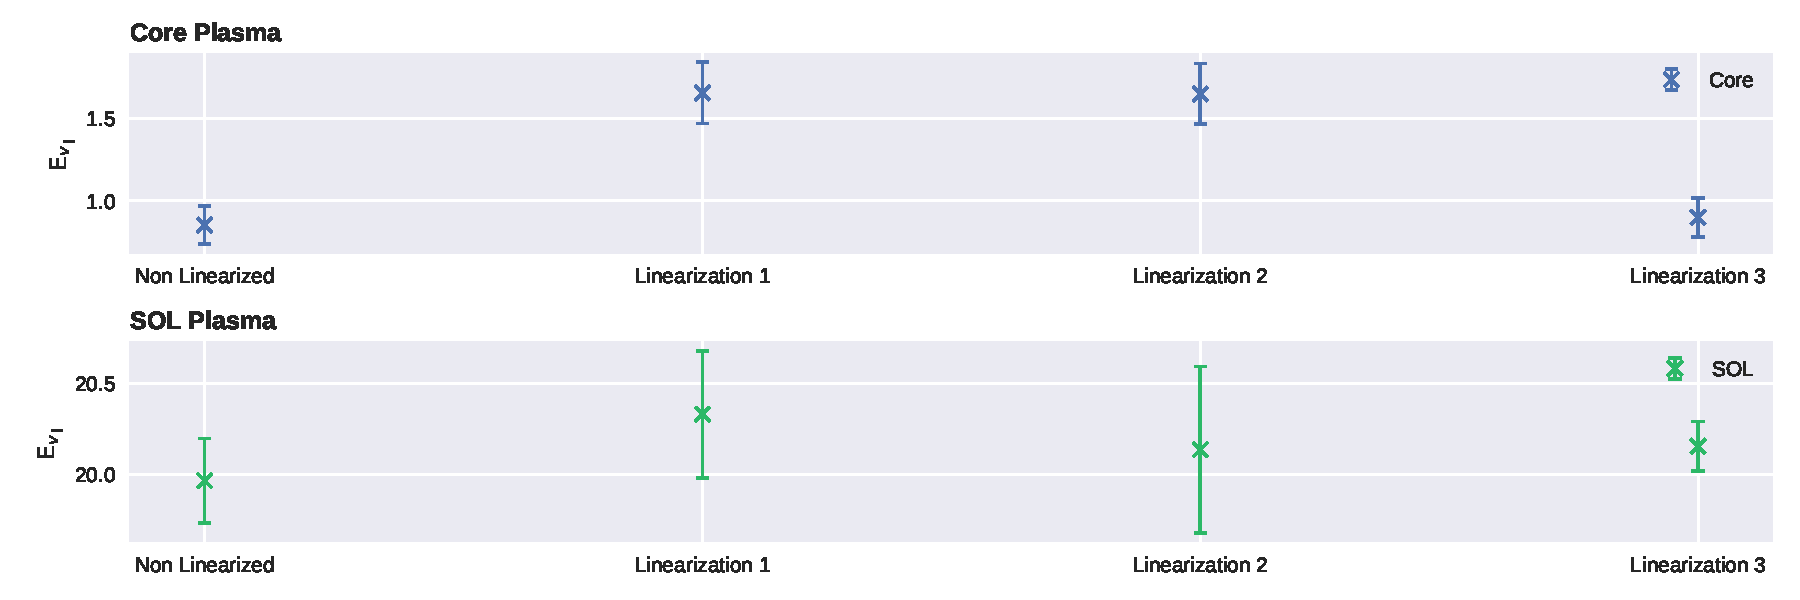
\includegraphics[width=0.5\linewidth]{pdfs/0-2_0-96/parallelvelocity_mean_100000.pdf}
    \caption{Zonal Profiles, mean Turbulent Flows and mean parallel Kinetic Energies for the 2\textsuperscript{nd} parameter set at low resolution $h_x = h_y = 1.0$. The mean values are taken from iteration 100,000 to 150,000.}
    \label{fig:low-resoultion-set-2}
\end{figure}



The two groups from the previous section are formed again, but this time more differences between them are visible. For instance the maximum zonal flow is achieved much close to the separatrix for the first group.\newline
Also for the turbulent flow and the parallel kinetic energies the two groups are visible again. As in the previous section the second group produces higher turbulent flows and parallel kinetic energies.\newline
For this parameter set the differences between the linearizations are generally more significant and for example the $\left< \overline{\Gamma} \right>$ in the Core region for the non linearized polarization equation is double the magnitude of the linearization one. As the only difference to the first parameter set is $\nu_\perp$ one can see that this parameter has different effects on the linearizations.\newline
Also for these parameters the turbulent flux for the first group is smaller compared to the first group in the Core region and vise versa in the \ac{SOL}.


\subsubsection{High Resoltion (8x256x1024 $h_x = h_y = 0.5$)}

The high resolution data for the 2\textsuperscript{nd} parameter set is persented in \autoref{fig:high-resoultion-set-2}

\begin{figure}[!hbtp]
    \textbf{Zonal Profiles, mean Turbulent flows and Parallel Kinetic Energies}\par\medskip
    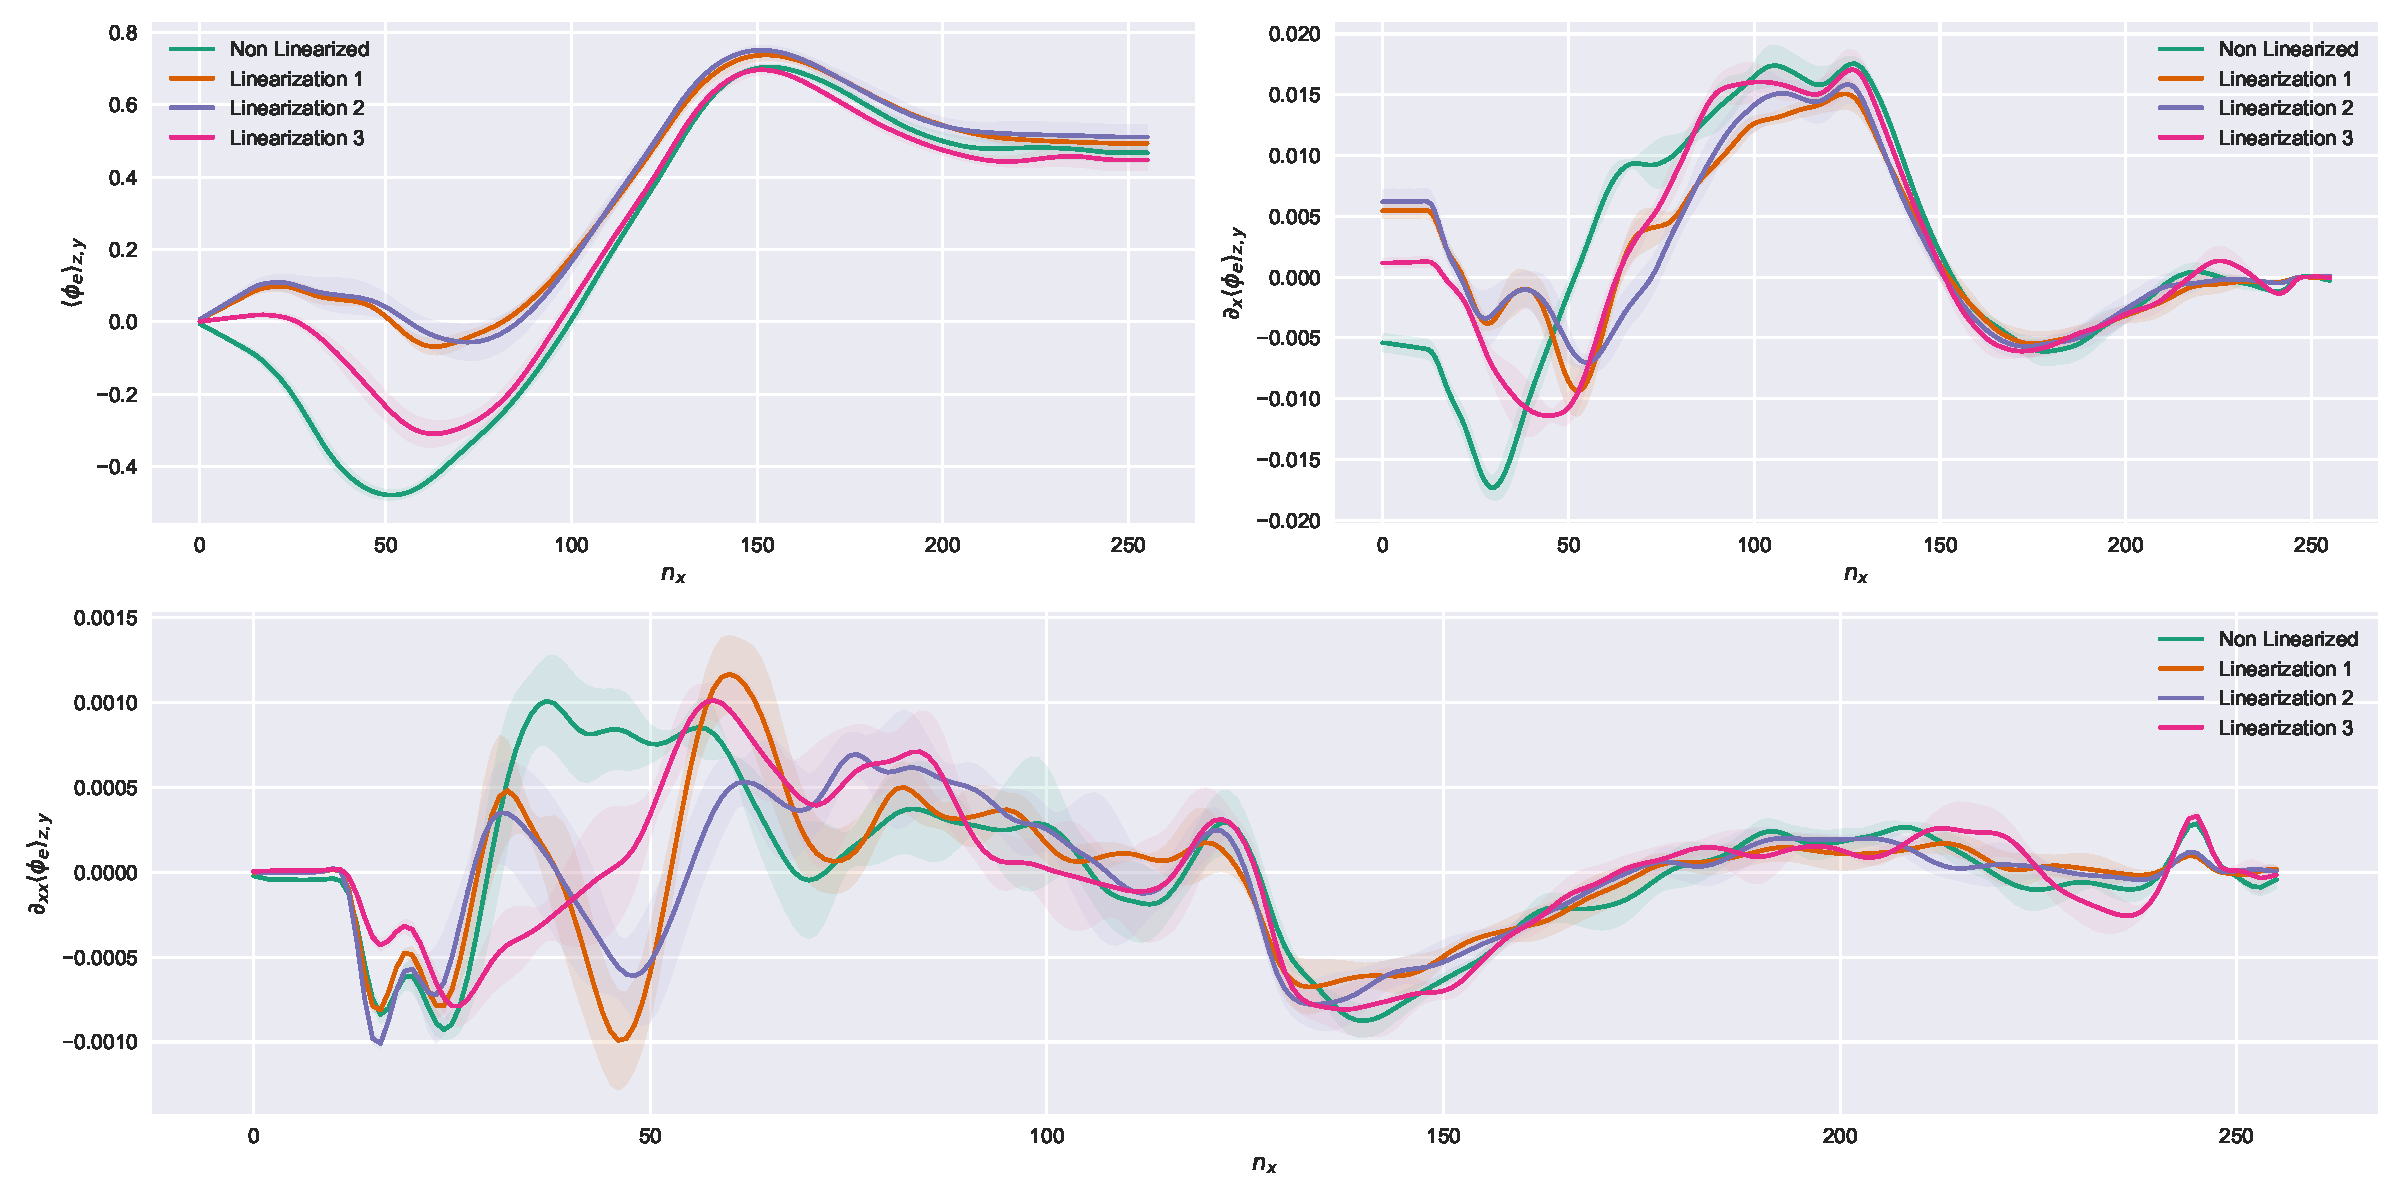
\includegraphics[width=\linewidth]{pdfs/0-2_0-06/zonal_profiles_100000.pdf}
    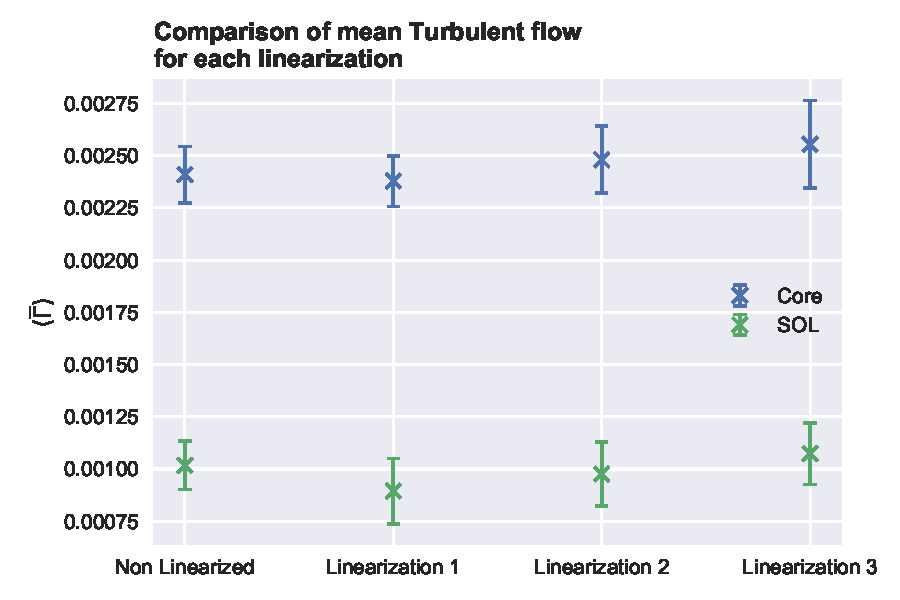
\includegraphics[width=0.5\linewidth]{pdfs/0-2_0-06/turbulent_flow_means_100000.pdf}
    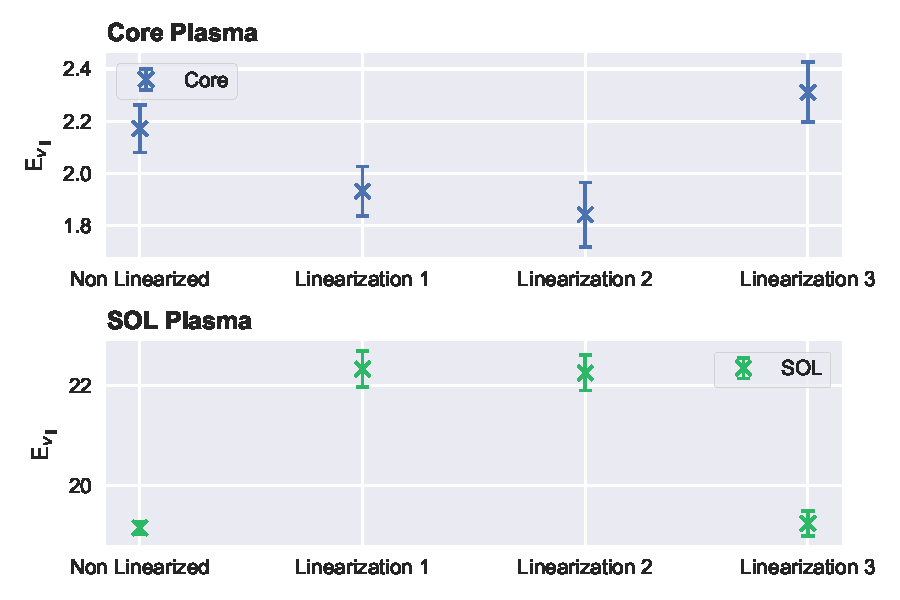
\includegraphics[width=0.5\linewidth]{pdfs/0-2_0-06/parallel_energies_100000.pdf}
    \caption{Zonal Profiles, mean Turbulent Flows and mean parallel Kinetic Energies for the 2\textsuperscript{nd} parameter set at higher resolution $h_x = h_y = 0.5$. The mean values are taken from iteration 100,000 to 150,000.}
    \label{fig:high-resoultion-set-2}
\end{figure}

The zonal profiles again show the formation of the second group but the first group now shows differences in the Core region ($0 < n_x \leq 128$) of the plasma. In this region there seems to be a strong effect of density fluctuations in the $y$-direction (which are better resolved by the non-linearized version). In the \ac{SOL} region there are no great differences visible especially when looking at the zonal flow and zonal vorticity. The turbulent flows now show no major differences but are more in line with the second group at low resolution than with the first. This can not be said for the parallel kinetic energies. The two groups greatly differ from each other. Interestingly there is an inversion of the differences between the two groups in the Core region in contrast to the low resolution data. Also the strong split between the two groups is not visible anymore in the zonal flow. It could be that at the low resolution combined with the high $\nu_\perp$ an important mode is supressed for the second group which is not the case for the first group. There are more differences visible for example when looking at the turbulent flux in the Core region which suggests that a resolution of $h_x=h_y=1.0$ is either not suitable or that for the higher resolution artificial modes play an important role.

\section{Resolution scaling of visocisity}

The 2\textsuperscript{nd} parameter set was also evaluated on a finer grid. This has some implications on the perpendicular hyperviscosity since this term is used to cut off high frequency modes in perpendicular direction. But since now the we have a finer resolution in that direction it is not necessary anymore to cut off these modes. Since we are using the fourth derivative in each direction for each direction we get a factor of 4 (in the Fourier-space) and because of that reduce $\nu_\perp$ by $\frac{1}{16} = \frac{1}{4\cdot4}$ to $\nu_\perp = 0.06$. $\nu_\parallel$ stays untouched since we didn't change the resolution in z-direction \footnote{It should be noted though that through magnetic shearing there could actually be an effect from higher perpendicular resolution on the parallel direction}. All other parameters exactly stay the same. The gathered data is shown in \autoref{fig:high-resoultion-set}. 


\section{Numerical stability}
Not thoroughly measured was the stability of the simulation but still some information will be presented here. For example if one increases the magnetic curvature to 0.05 for the lower resolution grid (leading to stronger turbulence) only the non linearized model is numerical stable. One has to deal with high gradients at the boundaries which seem to be a greater problem for the linearized models. 
Furthermore if the resolution is increased the $\Delta t$ has to be decreased but the non linearized model is still stable for higher $\Delta t$'s whereas the linearizations are much more sensitive to an increase of the resolution and need smaller $\Delta t$'s. It seems that the \ac{CFL} number is higher for the linearized models.

\section{Conclusion}

In this chapter the effects of the different linearizations where evaluated on a 3-dimensional grid representing the edge area of a tokamak using the Isothermal 3D Full-F Gyrofluid Model presented in \autoref{sec:isothermalequations}. The simulation was run for two different parameter sets. The first parameter set produced \textit{fine} looking results for a resolution in the size of the Ion gyro-radius ($h_x=h_y=1.0$). The second parameter set was chosen to validate the results on a higher resolution grid ($h_x=h_y=0.5$). This was necessary since transforming the first parameter set to a higher resolution was not possible because of artificial numerical effects that needed to be compensated by the viscosity terms (which weren't strong enough on the low resolution parameter set). The second parameter set was chosen such that it produces reasonable results\footnote{Considering stability and turbulent spectra.} for the higher resolution and then the set is \textit{transformed} for a lower resolution evaluation (this means adjusting the perpendicular hyperviscosity).\newline
As is expectable the polarization equation versions form two groups. The first group consists out of the non linearized version and the third linearization. Both of them still consider the background density gradient in $x$-direction where the second group (first and second linearization) both assume no gradient in the background density. This effect is mostly seen at the simulation boundaries where artificial strong gradients exist, but also in the core region. Especially the zonal profiles show greater deviations in the core region than in the SOL region.\newline
The second parameter set shows some unusual behavior and strong differences between the linearizations at the lower resolution which probably stems from the much higher perpendicular hyperviscosity. Because of that this data set should only be considered with caution.\newline
The low resolution sets are generally questionable since the viscosities need to be chosen very high to achieve a stable simulation. Because of that further on the discussion only relates to the second parameter set for the higher resolution.\newline
At this resolution the zonal profiles also show different results for the first group but this is mostly restricted to the Core region. This hints that in that region fluctuations in $y$-direction are of the size of the background whereas it does not seem to play major role in the \ac{SOL} region.  Generally the zonal profiles look very much the same beyond the separatrix (expect for the very boundary where numerical artifacts play a major role). The turbulent flow is of the same order for each linearization. This can not be said for the parallel kinetic energy. Here it looks like the first group concentrates more of $E_{v\parallel}$ in the Core region and the second group more in the \ac{SOL} region. In this region the effects of the limiter boundary conditions play a major role since they have a strong effect on $v_{\parallel}$. These differences suggest that the constant background linearizations should be used with caution when considering such boundary conditions.\newline
In the end there is definitely a difference visible for the different linearizations which may even be bigger for different parameters or resolutions.





\end{document}